\documentclass[%
11pt,%
%oneside,%
twoside,%
%twocolumn,%
titlepage,%
%fleqn,%
%a4page,%
german,%
headsepline%
]{scrartcl}

%\usepackage{fancyhdr}
%\usepackage{scrpage2}
\usepackage{lastpage}
\usepackage{geometry}
\usepackage{graphicx}
\usepackage[utf8]{inputenc}
\usepackage[ngerman]{babel}
\usepackage{lscape}
\usepackage[framemethod=TikZ]{mdframed}
\usepackage[most]{tcolorbox}
\usepackage{mymath}
\usepackage{units}
\usepackage{nicefrac}
\usepackage{pgf,tikz}
\usetikzlibrary{arrows}
\usepackage{colortbl}
\usepackage{hhline}
\usepackage{multirow}
\usepackage[extendedchars]{grffile}
\usepackage{caption}
\usepackage{multicol,calc}
\usepackage{blindtext}
\usepackage{pdfpages}
\usepackage{hyperref}
\usepackage[official]{eurosym}
\usetikzlibrary{arrows}
\usetikzlibrary{positioning}
\usetikzlibrary{shadows}

\usepackage{marginnote}
\usepackage{qrcode}
\qrset{height=9ex}

%\usepackage{romannum}
\usepackage{longtable}
\usepackage{listings}
\usepackage{wrapfig}


% Command, um Tabellen-Spalten anzupassen
\newcommand{\spaltenheight}{\rule{0mm}{3ex}}
\newcommand{\spaltenwidth}{\rule{3cm}{0mm}}
\newcommand{\spaltensep}{\\[1ex]}
%\arrayrulecolor{darkgreen}
\doublerulesepcolor{white}
\definecolor{lightyellow}{rgb}{1,1,0.8}
\definecolor{Gray}{gray}{0.9}


% Pagestyle/Layout
%\geometry{a4paper , tmargin =2.5cm,	bmargin=3cm, lmargin =2.5cm,	rmargin =2.5cm,	headheight=3em, headsep=1em, footskip=1cm}
\setlength{\parindent}{0pt} \setlength{\parskip}{1em}
%für TwoSide
%\lehead{\headmark\pagemark}
%\cehead{}
%\rehead{}
%\lohead{}
%\cohead{}
%\rohead{\headmark}
%für OneSide
%\ihead{}
%\chead{}
%\ohead{}
%\setheadsepline{0.5pt} % Linie zur Begrenzung
%\setfootsepline{0.5pt} % Linie zur Begrenzung
\pagestyle{headings} % gemachte Einstellungen anwenden

% Farbig umrahmte Umgebung Satz
 
 \definecolor{myblizzardblue}{HTML}{87CEEB}

\newcounter{satzz}[section]\setcounter{satzz}{0}
\renewcommand{\thesatz}{\arabic{section}.\arabic{satzz}}

\newenvironment{csatz}[2][]{%
    \refstepcounter{satzz}
 
    \ifstrempty{#1}%
    % if condition (without title)
    {\mdfsetup{%
        frametitle={%
            \tikz[baseline=(current bounding box.east),outer sep=0pt]
            \node[anchor=east,rectangle,fill=myblizzardblue]
            {\strut Satz~\thesatz};}
        }%
    % else condition (with title)
    }{\mdfsetup{%
        frametitle={%
            \tikz[baseline=(current bounding box.east),outer sep=0pt]
            \node[anchor=east,rectangle,fill=myblizzardblue]
            {\strut Satz~\thesatz:~#1};}%
        }%
    }%
% for both conditions
    \mdfsetup{%
        innertopmargin=10pt,linecolor=myblizzardblue,%
        backgroundcolor=whitesmoke,%
        linewidth=2pt,topline=true,%
        frametitleaboveskip=\dimexpr-\ht\strutbox\relax%
    }
 
\begin{mdframed}[]\relax}{%
\end{mdframed}}

% Farbig umrahmte Umgebung Theorem
 
\definecolor{mygraphblue}{HTML}{84B7E1}
\definecolor{whitesmoke}{HTML}{F5F5F5}

\newcounter{theo}[section]\setcounter{theo}{0}
\renewcommand{\thetheo}{\arabic{section}.\arabic{theo}}

\newenvironment{ctheo}[2][]{%
    \refstepcounter{theo}
 
    \ifstrempty{#1}%
    % if condition (without title)
    {\mdfsetup{%
        frametitle={%
            \tikz[baseline=(current bounding box.east),outer sep=0pt]
            \node[anchor=east,rectangle,fill=mygraphblue]
            {\strut Theorem~\thetheo};}
        }%
    % else condition (with title)
    }{\mdfsetup{%
        frametitle={%
            \tikz[baseline=(current bounding box.east),outer sep=0pt]
            \node[anchor=east,rectangle,fill=mygraphblue]
            {\strut Theorem~\thetheo:~#1};}%
        }%
    }%
% for both conditions
    \mdfsetup{%
        innertopmargin=10pt,linecolor=mygraphblue,%
        backgroundcolor=whitesmoke,%
        linewidth=2pt,topline=true,%
        frametitleaboveskip=\dimexpr-\ht\strutbox\relax%
    }
 
\begin{mdframed}[]\relax}{%
\end{mdframed}}

% Farbig umrahmte Umgebung Definition
 
 \definecolor{emerald}{HTML}{50C878}

\newcounter{deff}[section]\setcounter{deff}{0}
\renewcommand{\thedeff}{\arabic{section}.\arabic{deff}}

\newenvironment{cdef}[2][]{%
    \refstepcounter{deff}
 
    \ifstrempty{#1}%
    % if condition (without title)
    {\mdfsetup{%
        frametitle={%
            \tikz[baseline=(current bounding box.east),outer sep=0pt]
            \node[anchor=east,rectangle,fill=emerald]
            {\strut Definition~\thedeff};}
        }%
    % else condition (with title)
    }{\mdfsetup{%
        frametitle={%
            \tikz[baseline=(current bounding box.east),outer sep=0pt]
            \node[anchor=east,rectangle,fill=emerald]
            {\strut Definition~\thedeff:~#1};}%
        }%
    }%
% for both conditions
    \mdfsetup{%
        innertopmargin=10pt,linecolor=emerald,%
        backgroundcolor=whitesmoke,%
        linewidth=2pt,topline=true,%
        frametitleaboveskip=\dimexpr-\ht\strutbox\relax%
    }
 
\begin{mdframed}[]\relax}{%
\end{mdframed}}

% Farbig umrahmte Umgebung Achtung
 
 \definecolor{mygraphred}{HTML}{E26A6A}

\newcounter{merkee}[section]\setcounter{merkee}{0}
\renewcommand{\themerkee}{\arabic{section}.\arabic{merkee}}

\newenvironment{cachtung}[2][]{%
    \refstepcounter{merkee}
 
    \ifstrempty{#1}%
    % if condition (without title)
    {\mdfsetup{%
        frametitle={%
            \tikz[baseline=(current bounding box.east),outer sep=0pt]
            \node[anchor=east,rectangle,fill=mygraphred]
            {\strut Achtung};}
        }%
    % else condition (with title)
    }{\mdfsetup{%
        frametitle={%
            \tikz[baseline=(current bounding box.east),outer sep=0pt]
            \node[anchor=east,rectangle,fill=mygraphred]
            {\strut Achtung:~#1};}%
        }%
    }%
% for both conditions
    \mdfsetup{%
        innertopmargin=10pt,linecolor=mygraphred,%
        backgroundcolor=whitesmoke,%
        linewidth=2pt,topline=true,%
        frametitleaboveskip=\dimexpr-\ht\strutbox\relax%
    }
 
\begin{mdframed}[]\relax}{%
\end{mdframed}}

\subject{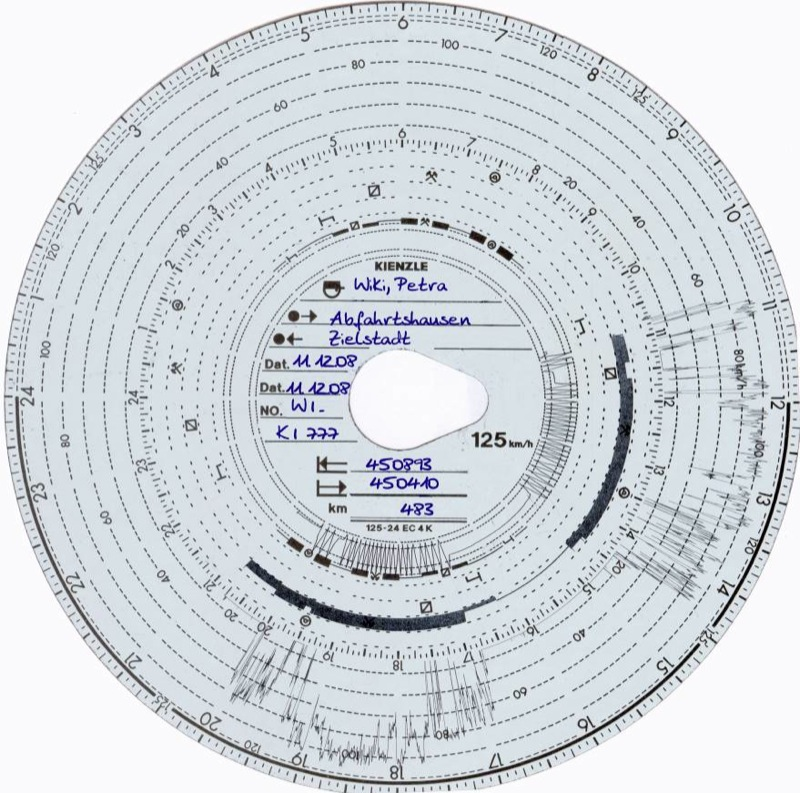
\includegraphics[width=0.618\textwidth]{pictures/tacho.jpg}}
\title{Integralrechnung}
\subtitle{Differenzialrechnung abrunden}
\author{}
\date{}
%\lowertitleback{
%\includegraphics[height=1.1cm]{/Users/jormawassmer/Pictures/logokoeniz.jpg}%
%\copyright Jorma Wassmer
%1. Auflage, Februar 2011
%}


\begin{document}
\maketitle
\tableofcontents
%\thispagestyle{empty}
\cleardoublepage
%\setcounter{page}{1}

\section{Was heisst Integral?}

Bei der Diskussion von Funktionen war bis anhin die Ableitung ein zentraler Begriff. Mit ihrer Hilfe kann man die momentane Änderungsrate einer Grösse bestimmen:
$$\lim_{x\rightarrow x_0}\frac{f(x)-f(x_0)}{x-x_0}.$$
Im Folgenden wird nun umgekehrt diskutiert, wie man von der momentanen Änderungsrate einer Grösse auf die Gesamtänderung der Grösse schliessen kann. Es stellt sich heraus, dass die Gesamtänderung einer Grösse als Flächeninhalt unter einer Kurve interpretiert werden kann. Deshalb sucht man nach Methoden zur Bestimmung solcher Flächeninhalte.

Lokomotiven, Cars oder Lastwagen müssen mit einem Fahrtenschreiber ausgerüstet sein, einem Messgerät, das zu jedem Zeitpunkt $t$ die momentane Geschwindigkeit $v(t)$ des Fahrzeugs aufzeichnet. Damit wird es den Untersuchungsbehörden im Falle eines Unglücks bzw. der Polizei bei einer Verkehrskontrolle ermöglicht festzustellen, wo sich das Fahrzeug zu einem bestimmten Zeitpunkt seiner Fahrt gerade befand, vorausgesetzt, dass seine Route und die Startzeit bekannt sind. Hauptsächlich wird überprüft, ob die Fahrer ihre gesetzlich vorgeschriebenen Ruhezeiten einhalten.

\begin{ueb}[Fahrtenschreiber]
Ermittle aus dem Fahrtenschreiber-Diagramm \ref{abb:schreiber} auf Seite \pageref{abb:schreiber}, mit welcher Geschwindigkeit das Fahrzeug um 17:15 Uhr und um 18:10 Uhr fuhr. Wann war das Fahrzeug nicht unterwegs?
\begin{figure}[h!t]
\begin{center}
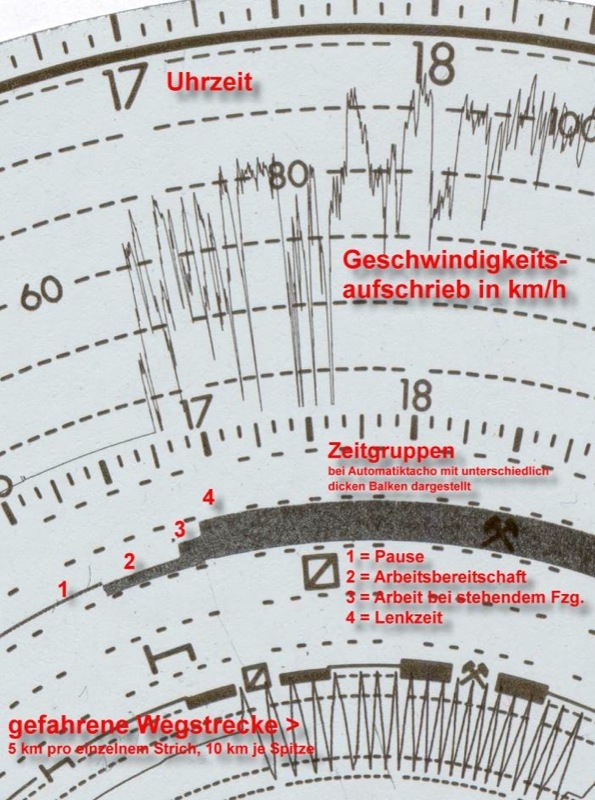
\includegraphics[width=0.381\textwidth]{pictures/tachozoom}
\end{center}
\caption{Fahrtenschreiber}\label{abb:schreiber}
\end{figure}
\end{ueb}

In der Differentialrechnung ermittelt man aus der Weg-Zeit-Funktion durch Differenziation die Geschwindigkeits-Zeit-Funktion
$$v(t) = \frac{\mathrm{d}s(t)}{\mathrm{d}t} = s'(t).$$
Allgemein gesprochen: Von einer gegebenen Funktion $f$ wird der Differentialquotient (bzw. die Ableitung $f'$) berechnet und dessen Eigenschaften untersucht. Dabei zeigt sich, dass nur die Funktionswerte in einer beliebig kleinen Umgebung von $x_0$ Einfluss auf den Wert des Differentialquotienten an dieser Stelle $x_0$ nehmen.

\begin{bem}
In der Differentialrechnung werden nur lokale Eigenschaften der Funktion untersucht.
\end{bem}

Das Beispiel mit dem Fahrtenschreiber verlangt aber genau umgekehrt die Rekonstruktion des Bewegungsverlaufes: Aus $v(t)$ soll $s(t)$ ermittelt werden.

In der Integralrechnung sucht man zu einer gegebenen Funktion $f$ die \glqq Antiableitung\grqq, also eine Funktion $F$, deren Ableitung gerade $f$ entspricht. Man muss aus den Änderungsdaten, die durch $f$ gegeben sind, die ursprüngliche Funk\-tion $F$ rekonstruieren. Durch diese Rekonstruktion kann der Gesamtzuwachs der Funktion, der Gesamteffekt ihrer Änderungen, berechnet werden.

Newton und Leibniz, die beiden Entdecker der Differentialrechnung trieben auch die hier vorgestellte \emph{Integralrechnung} voran. Die symbolische Schreibweise $\int$ geht auf Leibniz zurück, wobei dieses Zeichen an das Wort Summe (lat. \emph{fumma}, \glqq f\grqq\ steht für ein langes s) erinnern soll. Wie wir sehen werden, geht es nämlich in der Integralrechnung darum, infinitesimal kleine Flächenstücke aufzusummieren. Die Notation $f(x)\,\mathrm{d}x$ bedeutet die Fläche einer \glqq Säule\grqq\ mit Höhe $f(x)$ und infinitesimal kleiner Breite $\mathrm{d}x$.

\begin{bsps}
\ \\[-4ex]
\begin{itemize}
\item  Berechnung des zu jedem Zeitpunkt zurückgelegten
Weges, wenn die Ge\-schwin\-dig\-keits-Zeit-Funk\-tion
bekannt ist.
\item Berechnung der zu jedem Zeitpunkt erzielten Geschwindigkeit, wenn die Beschleunigungs-Zeit-Funktion bekannt ist.
\item Berechnung von Flächen- und Rauminhalten.
\item Berechnung von Schwerpunkten von Flächen und
Körpern.
\item Berechnung der Arbeit, wenn die wirkende Kraft als
Funktion des Weges bekannt ist.
\item Berechnung der Gesamtkosten, wenn die Grenzkosten jeweils bekannt sind.
\end{itemize}

\end{bsps}

\begin{bem}
In der Integralrechnung werden nicht lokale, sondern globale Eigenschaften einer Funktion untersucht.
\end{bem}

\begin{ueb}[Standardbeispiel]
Notiere für die gleichmässig beschleunigte Bewegung ($a=\text{konst}$) die Funk\-tions\-glei\-chungen für
\begin{enumeratea}
\item die zurückgelegte Strecke $s(t)$ in Abhängigkeit der Zeit.
\item die Geschwindigkeit $v(t)$ in Abhängigkeit der Zeit.
\item die Beschleunigung $a(t)$ in Abhängigkeit der Zeit.
\end{enumeratea}
und skizziere die Funktionen. Erkläre anschliessend den Zusammenhang zwischen $s(t)$, $v(t)$, und $a(t)$ und bestimme beim $v-t$- und $a-t$-Diagramm den Flächeninhalt zwischen dem entsprechenden Graphen und der $x$-Achse. Betrachte dazu das Zeitintervall $t\in [0,2]$ und setze $a=\unitfrac[2]{m}{s^2}$.
\end{ueb}

\section{Die Stammfunktion}
\begin{cdef}[Stammfunktion]{def:stammfunktion}
\marginnote{
\qrcode{
https://www.youtube.com/watch?v=VX4Ej4Haq44}
}
Gegeben
sei eine auf dem Intervall $I$ definierte Funktion $f$. $S(x)$ heisst \emph{Stammfunktion} von $f(x)$ im Intervall $I$, wenn $\frac{\mathrm{d}S}{\mathrm{d}x}=f$ für alle $x\in I$.
\end{cdef}

\begin{bem}
Salopp: $S$ ist Stammfunktion von $f$, wenn $S$ abgeleitet gleich $f$ ist:
$$S'(x)=f(x)$$
\end{bem}

\begin{bsps}
Beispiele von Stammfunktionen sind:
\begin{itemize}
\item $S(x)=\frac{x^3}{3}$ zu $f(x)=x^2$.
\item $S(x)=\frac{x^3}{3}+5$ zu $f(x)=x^2$.
\item $S(x)=-\cos(x)$ zu $f(x)=\sin(x)$
\end{itemize}
\end{bsps}

Das obige Beispiel zeigt auch, wieso ich in der Definition von \emph{einer} Stammfunktion von $f$ gesprochen habe. Weil nämlich beim Ableiten eine additive Konstante wegfällt, gibt es zu einer Funktion $f$ unendlich viele Stammfunktionen $S$. Man kann ja so viele verschiedene Konstanten hinzufügen wie es reelle Zahlen gibt. Wir halten dies kurz fest, in folgendem

\begin{csatz}{satz:inftystfktn}
Ist $S$ eine Stammfunktion von $f$, so gilt für alle weiteren Stammfunktionen $\tilde{S}$ von $f$:
$$\tilde{S}(x) = S(x) + c\q\text{mit }c\in\D{R}.$$
\end{csatz}

\begin{proof}
Man betrachtet die Funktion $H$ mit dem Funktionsterm $H(x) = F(x) - G(x)$, wobei $F$ und $G$ Stammfunktionen von $f$ sind. Also gilt für die Steigungsfunktion $H'(x) = F'(x) - G'(x) = f(x) - f(x) = 0$ und somit $H(x) = c$, da eine Funktion, deren Graph immer parallel zur $x$-Achse verläuft, notwendigerweise konstant sein muss.
\end{proof}

Man kann also zu einer Funktion $f$ beliebig viele Stammfunktionen angeben, wenn man zu irgendeiner Stammfunktion $F$ beliebige Konstanten addiert. In der Praxis ist es üblich, nur mit Repräsentanten aus der Menge
$$\setm{F(x) + c}{ F'(x) = f(x), c\in\mR},$$
der Menge aller Stammfunktionen der Funktion $f$, zu arbeiten.
Für den Zusammenhang Funktion - Stammfunktion benutzt man ein besonderes Symbol und schreibt:
$$\int f(x)\;\mathrm{d}x = F(x) + c$$
(lies: unbestimmtes Integral von $f(x)\;\mathrm{d}x =\dots$)

Das Symbol $\int\dots \mathrm{d}x$ steht für die Aufforderung, den Integranden $f$ zu integrieren (integrare, lat., wiederherstellen), also die Stammfunktion von $f$ zu bestimmen. Das $\mathrm{d}x$ gibt an, dass nach der Integrationsvariablen $x$ integriert werden soll, im Sinne von
$$\int f(x)\;\mathrm{d}x=\int f(t)\;\mathrm{d}t=\int f(u)\;du=\dots.$$

Also
$$\int x^2t\;\mathrm{d}x=\frac{x^3}{3}t+c,$$
hingegen
$$\int x^2t\;\mathrm{d}t=x^2\frac{t^2}{2}+c.$$
$c$ bezeichnet man als \textbf{Integrationskonstante}.

\begin{ueb}[Stammfunktion]
Ermittle zu $f$ eine Stammfunktion $F$ und benutze die Integralschreibweise. Bestätige dein Ergebnis durch entsprechende Differenziation.

\begin{minipage}{0.5\textwidth}
\begin{enumeratea}
\item $f(x)=-\frac{1}{2}x$
\item $f(x)=3$
\item $f(t)=t^3+3t^2-4t+1$
\item $f(u)=\frac{1}{\sqrt{u}}+\sqrt{u}$
\item $v(s)=(1-s)^3$
\end{enumeratea}
\end{minipage}
\begin{minipage}{0.5\textwidth}
\begin{enumeratea}
\setcounter{enumi}{5}
\item $f(x)=x^n,\q n\in\mZ\setminus\set{-1}$
\item $f(x)=(3x-2)^4+\sqrt{5x}$
\item $f(x)=\sin x+\sin\frac{x}{2}$
\item $f(x)=\frac{3}{x}$
\item $f(t)=e^t$
\end{enumeratea}
\end{minipage}
\end{ueb}

\begin{ueb}[Antiableitung]
Find the antiderivative $F$ of

\begin{minipage}{0.5\textwidth}
\begin{enumeratea}
\item $x\mapsto\frac{4}{x^2}-5x$ with $F(4)=25$.
\item $x\mapsto4x^3-3x^2+4x+5$ with $F(1)=3$.
\end{enumeratea}
\end{minipage}
\begin{minipage}{0.5\textwidth}
\begin{enumeratea}
\setcounter{enumi}{2}
\item $t\mapsto\cos t-\sin t$ with $F(\frac{\pi}{4})=0$.
\item $t\mapsto e^{3t}$ with $F(\ln 9)=0$.
\end{enumeratea}
\end{minipage}
\end{ueb}

\begin{ueb}[integrieren]
Berechne

\begin{minipage}{0.5\textwidth}
\begin{enumeratea}
\item $\int (ax^2+bx+c)\;\mathrm{d}x$
\item $\int x^2\cos\varphi\;\mathrm{d}\varphi$
\item $\int e^{-2t}\;\mathrm{d}t$
\end{enumeratea}
\end{minipage}
\begin{minipage}{0.5\textwidth}
\begin{enumeratea}
\setcounter{enumi}{3}
\item $\int\frac{\mathrm{d}x}{x-3}$
\item $\int xe^{x^2+1}\;\mathrm{d}x$
\item $\int\frac{u^2}{4u^3-3}\;\mathrm{d}u$
\end{enumeratea}
\end{minipage}
\end{ueb}

\begin{ueb}[Umkehrung]
Bestätige durch Differentiation

\begin{minipage}{0.5\textwidth}
\begin{enumeratea}
\item $\int (ax+b)^n\;\mathrm{d}x=\frac{(ax+b)^{n+1}}{a(n+1)}+C$
\item $\int \cos^2x\;\mathrm{d}x=\frac{1}{2}(x+\sin x\cos x)+C$
\end{enumeratea}
\end{minipage}
\begin{minipage}{0.5\textwidth}
\begin{enumeratea}
\setcounter{enumi}{2}
\item $\int\ln(x)\;\mathrm{d}x=x(\ln( x)-1)+C$
\item $\int x\ln (x)\;\mathrm{d}x=\frac{x^2}{4}(2\ln(x)-1)+C$
\end{enumeratea}
\end{minipage}
\end{ueb}

\begin{ueb}[Öl]
Ein auf ein Riff aufgelaufener Öltanker verliert durch ein Leck Öl. Der Ölteppich breitet sich ungefähr mit der Geschwindigkeit
$$\frac{dR}{\mathrm{d}t}=\frac{8}{\sqrt{t}},\q t\geq1$$
radial aus, wobei $R(t)$ den Radius des kreisförmigen Ölteppichs in Meter nach $t$ Minuten angibt. Nach einer Minute beträgt der Radius bereits 15 Meter. Berechne den Radius nach 49 Minuten.
\end{ueb}

Nachdem für einige Funktionen bereits die Stammfunktionen konkret gebildet wurden, soll an dieser Stelle darauf hingewiesen werden, dass es in diesem Zusammenhang zwei grundsätzliche Fragen gibt:

\begin{itemize}
\item Gibt es zu \emph{jeder} Funktion $f$ eine Stammfunktion $F$, d.h. ist jede Funktion integrierbar?
\item Ist gegebenenfalls diese Stammfunktion auch berechenbar, d.h. kann man ihren Funk\-tions\-term \emph{explizit} angeben?
\end{itemize}

Ohne Beweis wollen wir lediglich zur ersten Frage bemerken: Jede auf einem abgeschlossenen Intervall stetige Funktion ist auf entsprechenden Intervall auch integrierbar.

\section{Das bestimmte Integral}
\subsection{Flächenberechnung als Grenzwertprozess}
Die
\marginnote{
\qrcode{
https://www.youtube.com/watch?v=76c9Zi-plTI}
}
Flächenberechnung, auch Integralrechnung genannt, befasst sich mit der Bestimmung krummlinig begrenzter Ebenenstücke. Dabei müssen die krummlinigen Grenzen als Graphen von Funktionen bekannt sein.
\begin{bsp}
Berechnen der Fläche zwischen dem Graphen von $f(x)=x^2$ und der x-Achse im Intervall $[0,1]$. Wir approximieren den gesuchten Flächeninhalt mit $n$ Rechtecken der Breite $\frac{1}{n}$ für ein festes $n\in\D{N}$, welche dem gesuchten Ebenenstück einbeschrieben sind. Wir erhalten nach kurzer Rechnung
$$U_n=\frac{(n-1)(2n-1)}{6n^2}.$$
Um eine bessere Näherung zu erhalten, lassen wir $n$ gegen Unendlich streben:
$$\lim_{n\rightarrow\infty} U_n = \frac{1}{3}.$$
Das bedeutet, dass der gesuchte Flächeninhalt mindestens ein Drittel beträgt. Nun nähern wir die gesuchte Fläche mit Rechtecken an, in welchen der Graph vollständig enthalten ist:
$$O_n=U_n+\frac{1}{n}\cdot 1.$$
Wiederum lassen wir $n$ gegen Unendlich streben:
$$\lim_{n\rightarrow\infty} O_n = \frac{1}{3}.$$
Das heisst, dass die Fläche höchstens $\frac{1}{3}$ beträgt. Zusammen mit dem ersten Resultat also, dass die gesuchte Fläche exakt $\frac{1}{3}$ beträgt.
\end{bsp}

\noindent $U_n$ nennt man sinnigerweise Untersumme und $O_n$ Obersumme. Hier die Darstellungen von $U_5$ und $O_5$ angewendet auf $f(x)=x^2$ im Intervall $[0,1]$.\\

\begin{figure}[h!t]
\definecolor{zzttqq}{rgb}{0.6,0.2,0}
\begin{tikzpicture}[line cap=round,line join=round,>=triangle 45,x=3.7cm,y=3.47cm]
\draw[->,color=black] (-0.4,0) -- (1.4,0);
\foreach \x in {-0.2,0.2,0.4,0.6,0.8,1,1.2}
\draw[shift={(\x,0)},color=black] (0pt,2pt) -- (0pt,-2pt) node[below] {\footnotesize $\x$};
\draw[color=black] (1.34,0.02) node [anchor=south west] {$x$};
\draw[->,color=black] (0,-0.4) -- (0,1.4);
\foreach \y in {-0.2,0.2,0.4,0.6,0.8,1,1.2}
\draw[shift={(0,\y)},color=black] (2pt,0pt) -- (-2pt,0pt) node[left] {\footnotesize $\y$};
\draw[color=black] (0.02,1.32) node [anchor=west] {$y$};
\draw[color=black] (0pt,-10pt) node[right] {\footnotesize $0$};
\clip(-0.4,-0.4) rectangle (1.4,1.4);
\draw[color=zzttqq,fill=zzttqq,fill opacity=0.1] (0,0) rectangle (0.2,0);
\draw[color=zzttqq,fill=zzttqq,fill opacity=0.1] (0.2,0) rectangle (0.4,0.04);
\draw[color=zzttqq,fill=zzttqq,fill opacity=0.1] (0.4,0) rectangle (0.6,0.16);
\draw[color=zzttqq,fill=zzttqq,fill opacity=0.1] (0.6,0) rectangle (0.8,0.36);
\draw[color=zzttqq,fill=zzttqq,fill opacity=0.1] (0.8,0) rectangle (1,0.64);
\draw[line width=1.2pt, smooth,samples=100,domain=0.0:1.4] plot(\x,{\x^2});
\draw[color=zzttqq] (0.4,1) node {$a = 0.24$};
\end{tikzpicture}
\hfill
\definecolor{zzttqq}{rgb}{0.6,0.2,0}
\begin{tikzpicture}[line cap=round,line join=round,>=triangle 45,x=3.7cm,y=3.45cm]
\draw[->,color=black] (-0.4,0) -- (1.4,0);
\foreach \x in {-0.2,0.2,0.4,0.6,0.8,1,1.2}
\draw[shift={(\x,0)},color=black] (0pt,2pt) -- (0pt,-2pt) node[below] {\footnotesize $\x$};
\draw[color=black] (1.34,0.02) node [anchor=south west] {$x$};
\draw[->,color=black] (0,-0.4) -- (0,1.4);
\foreach \y in {-0.2,0.2,0.4,0.6,0.8,1,1.2}
\draw[shift={(0,\y)},color=black] (2pt,0pt) -- (-2pt,0pt) node[left] {\footnotesize $\y$};
\draw[color=black] (0.02,1.32) node [anchor=west] {$y$};
\draw[color=black] (0pt,-10pt) node[right] {\footnotesize $0$};
\clip(-0.4,-0.4) rectangle (1.4,1.4);\draw[color=zzttqq,fill=zzttqq,fill opacity=0.1] (0,0) rectangle (0.2,0.04);
\draw[color=zzttqq,fill=zzttqq,fill opacity=0.1] (0.2,0) rectangle (0.4,0.16);
\draw[color=zzttqq,fill=zzttqq,fill opacity=0.1] (0.4,0) rectangle (0.6,0.36);
\draw[color=zzttqq,fill=zzttqq,fill opacity=0.1] (0.6,0) rectangle (0.8,0.64);
\draw[color=zzttqq,fill=zzttqq,fill opacity=0.1] (0.8,0) rectangle (1,1);
\draw[line width=1.2pt, smooth,samples=100,domain=0.0:1.4] plot(\x,{\x^2});
\draw[color=zzttqq] (0.4,1) node {$a = 0.44$};
\end{tikzpicture}
\caption{Unter- und Obersumme von $x^2$ über $[0,1]$ mit Schrittweite $0.2$}
\end{figure}

Wenn, wie in unserem Beispiel, Ober- und Untersumme für $n$ gegen Unendlich gegen den gleichen Wert konvergieren, dann sagt man:
\begin{quote}
\glqq Das Integral von $f(x)=x^2$ auf dem Intervall $[0,1]$ existiert und hat den Wert $\frac{1}{3}$\grqq.
\end{quote}

\begin{figure}
\begin{center}
\definecolor{zzttqq}{rgb}{0.6,0.2,0}
\begin{tikzpicture}[line cap=round,line join=round,>=triangle 45,x=3.7cm,y=3.45cm]
\draw[->,color=black] (-0.4,0) -- (1.4,0);
\foreach \x in {-0.2,0.2,0.4,0.6,0.8,1,1.2}
\draw[shift={(\x,0)},color=black] (0pt,2pt) -- (0pt,-2pt) node[below] {\footnotesize $\x$};
\draw[color=black] (1.35,0.01) node [anchor=south west] {$x$};
\draw[->,color=black] (0,-0.4) -- (0,1.4);
\foreach \y in {-0.2,0.2,0.4,0.6,0.8,1,1.2}
\draw[shift={(0,\y)},color=black] (2pt,0pt) -- (-2pt,0pt) node[left] {\footnotesize $\y$};
\draw[color=black] (0.02,1.33) node [anchor=west] {$y$};
\draw[color=black] (0pt,-10pt) node[right] {\footnotesize $0$};
\clip(-0.4,-0.4) rectangle (1.4,1.4);
\draw[color=zzttqq,fill=zzttqq,fill opacity=0.1, smooth,samples=50,domain=0.0:1.0] plot(\x,{\x^2}) -- (1,0) -- (0,0) -- cycle;
\draw[line width=1.6pt, smooth,samples=100,domain=0.0:1.4] plot(\x,{\x^2});
\draw[color=zzttqq] (0.4,0.8) node {$a=\frac{1}{3}$};
\end{tikzpicture}
\caption{Fläche unter $x^2$ über $[0,1]$}
\end{center}
\end{figure}

\begin{ueb}[Zwischensummen]
Berechne die Fläche zwischen $f(x)=x^2$ und der x-Achse auf dem Intervall $[0,b]$ mit $b\geq0$. Sie dürfen annehmen, dass Ober- und Untersumme gegen den gleichen Wert konvergieren. Für Interessierte: Welche Eigenschaft muss $f$ haben, damit sicher $O_\infty=U_\infty$?
\end{ueb}

\begin{ueb}[Zwischensummen 2]
Berechne die Fläche zwischen $f(x)=x^2$ und der x-Achse auf dem Intervall $[a,b]$ mit $a,b\in\D{R}^+_0, a\leq b$.
\end{ueb}

\begin{ueb}[Stammfunktion]
Zeichne den Graphen von $g(x)=x$. Berechne die Flächenfunktion $G(x)$ zwischen dem Graphen von $g$ und der x-Achse auf dem Intervall $[0,x]$, welche den Wert der Fläche in Abhängigkeit von $x$ angibt. Welcher Zusammenhang besteht zwischen $g$ und $G$?
\end{ueb}

\begin{ueb}[hoch 3]
Finde die Flächenformel $H$ für den Wert der Fläche zwischen dem Graphen $h(x)=x^3$ und der x-Achse auf dem Intervall $[a,b]$. $H$ hängt natürlich von $a$ und $b$ ab: $H(a,b)$.
\begin{center}

\definecolor{zzttqq}{rgb}{0.6,0.2,0}
\scalebox{0.70}{
\begin{tikzpicture}[line cap=round,line join=round,>=triangle 45,x=1.0cm,y=0.06cm]
\draw[->,color=black] (-2,0) -- (5,0);
\foreach \x in {-2,-1,1,2,3,4}
\draw[shift={(\x,0)},color=black] (0pt,2pt) -- (0pt,-2pt);
\draw[color=black] (4.8,0.6) node [anchor=south west] {$x$};
\draw[->,color=black] (0,-10) -- (0,80);
\foreach \y in {-10,10,20,30,40,50,60,70}
\draw[shift={(0,\y)},color=black] (2pt,0pt) -- (-2pt,0pt);
\draw[color=black] (0.06,77) node [anchor=west] {$y$};
\clip(-2,-10) rectangle (5,80);
\draw[color=zzttqq,fill=zzttqq,fill opacity=0.1, smooth,samples=50,domain=1.7:3.8] plot(\x,{\x^3}) -- (3.8,0) -- (1.7,0) -- cycle;
\draw[line width=1.2pt, smooth,samples=100,domain=-2.0:5.0] plot(\x,{\x^3});
\draw[color=zzttqq] (3.04,7) node {$H(a,b)$};
\draw[color=black] (1.7,-2.3) node {$a$};
\draw[color=black] (3.8,-2) node {$b$};
\end{tikzpicture}
}
\end{center}
\end{ueb}

\begin{bem}
Wir vermuten, dass für die Fläche unter $f(x)=x^n$ zwischen $a$ und $b$ gilt:
$$F = \frac{b^{n+1}}{n+1}-\frac{a^{n+1}}{n+1}.$$
\end{bem}

\subsection{Konventionen}
Ich werde im Folgenden etwas lascher in der Genauigkeit der Aussagen. Beispielsweise spreche ich oft nur von der Fläche unterhalb des Graphen von $f$ über dem Intervall $[a,b]$, meine damit aber die Fläche zwischen dem Graphen von $f$, der x-Achse und den Parallelen zur $y$-Achse durch $x=a$ und $x=b$. Oder etwa ist das Intervall $[a,b]$ natürlich so zu verstehen, dass $a\leq b$. Ausnahmen werden explizite angegeben.

\subsection{Definition}
Wir verallgemeinern das oben angewandte Verfahren auf die Fläche unter dem Graphen einer beliebigen Funktion $f$ zwischen $a$ und $b$. Statt der Rechtecke, die vollständig unterhalb bzw. oberhalb des Graphen liegen, nehmen wir solche, die einen Funktionswert auf dem entsprechenden Teilintervall als Höhe haben. Man spricht in diesem Fall von einer \textbf{Zwischenrechtecksumme} $Z_n$. Diese $Z_n$ bilden für $n\in\D{N}$ eine Folge, welche für $n\rightarrow\infty$ gegen den Wert der Fläche unter dem Graphen von $f$ strebt.

\begin{cdef}[Bestimmtes Integral]{}
Wenn alle Zwischensummenfolgen des Graphen von $f$ gegen den gleichen Grenzwert konvergieren, so heisst die Funktion $f$ über $[a,b]$ \emph{integrierbar}. Der gemeinsame Grenzwert heisst \emph{bestimmtes Integral} von $f$ über $[a,b]$, und man schreibt:
$$\int_a^b f(x)\,\mathrm{d}x$$
$a$ und $b$ heissen \emph{Integralgrenzen}.
\end{cdef}

\begin{bem}
Das Integralzeichen $\int$ ist ein stilisiertes \texttt{S}, in Anlehnung an die Berechnung durch Zwischen\emph{summen}.
\end{bem}

\section{Der Hauptsatz der Differential- und Integralrechnung}
Bevor wir auf den Hauptsatz zu sprechen kommen, führen wir hilfreiche Begriffe ein.

\begin{cdef}[Integralfunktion]{}
Unter der \emph{Integralfunktion} einer integrierbaren Funktion $f$ versteht man die Funktion
$$I(x) = \int_a^xf(t)\;\mathrm{d}t.$$
\end{cdef}

\begin{ueb}[Integralfunktion]
Bestimmen Sie die Integralfunktion von

\begin{minipage}{2.5cm}
\begin{enumeratea}
\item $f(x)=x^2$
\end{enumeratea}
\end{minipage}
\begin{minipage}{2.5cm}
\begin{enumeratea}
\addtocounter{enumi}{1}
\item $g(x)=x^3$
\end{enumeratea}
\end{minipage}
\begin{minipage}{2.5cm}
\begin{enumeratea}
\addtocounter{enumi}{2}
\item $h(x)=x$
\end{enumeratea}
\end{minipage}

\end{ueb}

Die Beispiele aus obiger Übung lassen vermuten:

\begin{csatz}[Hauptsatz der Integral- \& Differentialrechnung]{satz:hauptsatz}
Die Integralfunktion jeder stetigen Funktion ist differenzierbar. Ihre Ableitung ist gleich der Integrandfunktion.
\end{csatz}\label{satz:hauptsatz}

\begin{proof}[Beweis]
Eine Möglichkeit, diesen Satz zu beweisen, geht vom Differenzenquotienten der Integralfunktion  aus:
$$I'(x) = \lim_{h\rightarrow0} \frac{I(x+h)-I(x)}{h}.$$
Jetzt schreibt man $I$ explizite
$$I'(x) = \lim_{h\rightarrow0} \frac{\int_a^{x+h}f(t)\;\mathrm{d}t-\int_a^xf(t)\;\mathrm{d}t}{h}$$
und wendet die Integraladditivität an, wobei $l$ die Höhe des Zwischensummenrechtecks mit Breite $h$ auf dem Intervall $[x,x+h]$ bezeichnet:
\begin{align*}
I'(x) &= \lim_{h\rightarrow0} \frac{\int_x^{x+h}f(t)\;\mathrm{d}t}{h}=\lim_{h\rightarrow0}\frac{hl}{h}\\
&=\lim_{h\rightarrow0}l=f(x),
\end{align*}
da für $h\rightarrow0$ wegen der Stetigkeit von $f$ $l$ gegen $f(x)$ strebt.
\end{proof}

\begin{figure}[h!t]
\begin{center}
\definecolor{ffcccc}{rgb}{1,0.8,0.8}
\definecolor{zzttqq}{rgb}{0.6,0.2,0}
\definecolor{ccqqtt}{rgb}{0.8,0,0.2}
\begin{tikzpicture}[line cap=round,line join=round,>=triangle 45,x=0.5cm,y=1cm]
\draw[->,color=black] (-1.86,0) -- (8.92,0);
\foreach \x in {-1,1,2,3,4,5,6,7,8}
\draw[shift={(\x,0)},color=black] (0pt,2pt) -- (0pt,-2pt);
\draw[color=black] (8.4,0.08) node [anchor=south west] { x};
\draw[->,color=black] (0,-1.08) -- (0,4.5);
\foreach \y in {-1,1,2,3,4}
\draw[shift={(0,\y)},color=black] (2pt,0pt) -- (-2pt,0pt);
\draw[color=black] (0.1,4.1) node [anchor=west] { y};
\clip(-1.86,-1.08) rectangle (8.92,4.5);
\fill[color=zzttqq,fill=zzttqq,fill opacity=0.05] (4,2.98) -- (6,2.98) -- (6,0) -- (4,0) -- cycle;
\draw[color=ffcccc,fill=ffcccc,fill opacity=0.05, smooth,samples=50,domain=1.2:4.0] plot(\x,{ln(\x+2)+1}) -- (4,0) -- (1.2,0) -- cycle;
\draw[line width=1.2pt, smooth,samples=100,domain=-1.86:8.92] plot(\x,{ln(\x+2)+1});
\draw (0.8,-0.05) node[anchor=north west] {$a$};
\draw (3.5,-0.05) node[anchor=north west] {$x$};
\draw (5.1,0.03) node[anchor=north west] {$x+h$};
\draw [line width=1.2pt] (1.2,2.16)-- (1.2,0);
\draw [line width=1.2pt,color=ccqqtt] (4,2.98)-- (4,0);
\draw [line width=1.2pt,color=ccqqtt] (4,2.98)-- (6,2.98);
\draw [line width=1.2pt,color=ccqqtt] (6,2.98)-- (6,0);
\draw [line width=1.2pt] (5,2.98)-- (5,0);
\draw [color=zzttqq] (4,2.98)-- (6,2.98);
\draw [color=zzttqq] (6,2.98)-- (6,0);
\draw [color=zzttqq] (6,0)-- (4,0);
\draw [color=zzttqq] (4,0)-- (4,2.98);
\draw (5.0,1.8) node[anchor=north west] {$I$};
\draw[color=black] (-0.9,1.7) node {$f(t)$};
\end{tikzpicture}
\end{center}
\caption{Zum Beweis des Hauptsatzes der Integral- und Differentialrechnung}
\end{figure}

Satz \ref{satz:hauptsatz} wird in der Literatur oft als Hauptsatz der Integral- und Differentialrechnung bezeichnet. Für unsere Zwecke aber möchte ich den nächsten Satz als Hauptsatz auszeichnen. 

Wir erhalten praktisch gratis mit obigem Beweis von Satz \ref{satz:hauptsatz} folgenden

\begin{csatz}[Flächenberechnung]{satz:obenminusunten}
Ist
\marginnote{
\qrcode{
https://www.youtube.com/watch?v=uo_JVS-OMsk}
}
$S(x)$ eine Stammfunktion der stetigen Funktion $f$, so gilt:
$$\int_a^bf(x)\,\mathrm{d}x = S(b) - S(a).$$
\end{csatz}
\begin{proof}[Beweis]
Man zeigt ganz leicht, dass die additive Konstante wegfällt.
\end{proof}

\begin{bem}
Dies ist der Hauptsatz der Differential- und Integralrechnung für einen Maturanden. Der Satz offenbart uns folgendes Rezept zur Flächenberechnung zwischen einem Graphen mit Funktionsgleichung $f$ und der x-Achse im Intervall $[a,b]$, ohne Grenzwerte beiziehen zu müssen:
\begin{enumerate}
\item Man bestimmt eine Stammfunktion $S$ der Integrandfunktion $f$.
\item Man bestimmt die Werte dieser Stammfunktion für $x=a$ und $x=b$.
\item Die Differenz dieser Werte, $S(b)-S(a)$, ist gleich dem bestimmten Integral.
\end{enumerate}

Man schreibt:
$$\int_a^bf(x)\,\mathrm{d}x=S(x)\,|^b_a=S(b)-S(a)$$
\end{bem}

Es genügt ein
\begin{bsp}
\begin{align*}
\int_0^{\frac{\pi}{2}}\sin(x)\,\mathrm{d}x&=-\cos(x)\,|_0^{\frac{\pi}{2}}\\
&=-\cos(\frac{\pi}{2})-(-\cos(0))\\
&=0-(-1)=1
\end{align*}
\end{bsp}

Halten Sie sich bei den Rechnungen an die Schreibweise, die im obigen Beispiel verwendet wird.
\begin{ueb}[Flächeninhalt]
Skizziere und berechne den Flächeninhalt unter $f(x)=\cos(x)$ zwischen $0$ und $\frac{\pi}{2}$.
\end{ueb}

\begin{ueb}[Fläche]
Berechne den Flächeninhalt unter $f(x)=x^4$ zwischen $1$ und $2$.
\end{ueb}

\begin{ueb}[integriere]
Achte jeweils darauf, ob der Integrand im Integrationsintervall überhaupt definiert ist, und berechne:

\begin{minipage}{0.4\textwidth}
\begin{enumeratea}
\item $\int_1^42\;\mathrm{d}x$
\item $\int_{-3}^8\;\mathrm{d}x$
\item $\int_{-5}^0(3-u)^2\;\mathrm{d}u$
\item $\int_{0.001}^{0.1}\frac{1}{x^2}\;\mathrm{d}x$
\item $\int_{-1}^1\frac{\mathrm{d}u}{u^2}$
\item $\int_1^9(2\sqrt{x}-\frac{3}{\sqrt{x}})\;\mathrm{d}x$
\end{enumeratea}
\end{minipage}
\begin{minipage}{3.9cm}
\begin{enumeratea}
\addtocounter{enumi}{6}
\item $\int_{-3}^{-1}\frac{1+t}{t^3}\;\mathrm{d}t$
\item $\int_0^\pi\sin x\;\mathrm{d}x$
\item $\int_\frac{1}{2}^2\frac{1}{x}\;\mathrm{d}x$
\item $\int_0^1t\mathrm{e}^{-t^2}\;\mathrm{d}t$
\item $\int_0^\frac{\pi}{2}\frac{\sin x}{1+2\cos x}\;\mathrm{d}x$
\item $\int_0^1\frac{1}{2}(\mathrm{e}^x+\mathrm{e}^{-x})\;\mathrm{d}x$
\end{enumeratea}
\end{minipage}
\end{ueb}

\begin{ueb}[Grenzen]
Berechne $b$ aus:

\begin{minipage}{0.4\textwidth}
\begin{enumeratea}
\item $\int_0^bt^2\;\mathrm{d}t=72$
\item $\int_1^b\frac{1}{x^2}\;\mathrm{d}x=\frac{3}{7}$
\end{enumeratea}
\end{minipage}
\begin{minipage}{7cm}
\begin{enumeratea}
\addtocounter{enumi}{2}
\item $\int_0^b(8t+2\sin t)\;\mathrm{d}t=\pi^2+2$
\item $\int_\mathrm{e}^b\frac{\mathrm{d}u}{u}=1$
\end{enumeratea}
\end{minipage}
\end{ueb}

\subsection{Existenz bestimmter Integrale}
Die Anwendung der Definition bestimmter Integrale ist im allgemeinen schwierig. Es gilt aber der folgende
\begin{csatz}{satz:integrierbar}
Jede über $[a,b]$ stetige Funktion $f$ ist über diesem Intervall auch integrierbar.
\end{csatz}

\begin{bem}\label{zusammenhang}
Zwischen Differenzierbarkeit, Stetigkeit und Integrierbarkeit besteht folgender Zusammenhang:
\begin{itemize}
\item Jede differenzierbare Funktion ist stetig, und jede stetige Funktion ist integrierbar.
\item Es gibt stetige Funktionen, die nicht differenzierbar sind.
\item Es gibt integrierbare Funktionen, die nicht stetig sind.
\item Es gibt Funktionen, die nicht integrierbar sind.
\end{itemize}
\end{bem}

\begin{ueb}[Spezialfälle]
Finde charakteristische Beispiele zu den Aussagen aus obiger Bemerkung.
\end{ueb}

\subsection{Flächen zwischen zwei Graphen}
Wir haben bereits gesehen, dass sich auch krummlinig begrenzte Flächen zwischen zwei Graphen, deren Funktionsgleichungen bekannt sind, leicht berechnet werden können.

Man zeichne sich ein Bildchen und folgender Satz ist anschaulich völlig klar:
\begin{csatz}{satz:flaechezwischen}
Für die Fläche zwischen zwei Graphen der Funktionen $f$ und $g$ im Intervall $[a,b]$ --- wobei wir ohne Einschränkung der Allgemeinheit annehmen können, dass $f(x)\geq g(x)$ für alle $x\in[a,b]$ ist --- gilt:
$$F = \int_a^bf(x)\,\mathrm{d}x - \int_a^bg(x)\,\mathrm{d}x$$
\end{csatz}

\begin{figure}[h!t]
\begin{center}
\definecolor{zzttqq}{rgb}{0.6,0.2,0}
\definecolor{qqwwcc}{rgb}{0,0.4,0.8}
\definecolor{uququq}{rgb}{0.25,0.25,0.25}
\begin{tikzpicture}[line cap=round,line join=round,>=triangle 45,x=0.5cm,y=0.5cm]
\draw[->,color=black] (-2,0) -- (11,0);
\foreach \x in {-2,-1,1,2,3,4,5,6,7,8,9,10}
\draw[shift={(\x,0)},color=black] (0pt,2pt) -- (0pt,-2pt);
\draw[color=black] (10.66,0.08) node [anchor=south west] { x};
\draw[->,color=black] (0,-2) -- (0,8);
\foreach \y in {-2,-1,1,2,3,4,5,6,7}
\draw[shift={(0,\y)},color=black] (2pt,0pt) -- (-2pt,0pt);
\draw[color=black] (0.1,7.6) node [anchor=west] { y};
\clip(-2,-2) rectangle (11,8);
\draw[color=zzttqq,fill=zzttqq,fill opacity=0.1] {[smooth,samples=50,domain=1.58:7.47] plot(\x,{ln(\x)+3})} -- (7.47,5.01) {[smooth,samples=50,domain=7.47:1.58] -- plot(\x,{0.25*(\x-4)^2+2})} -- (1.58,3.46) -- cycle;
\draw[line width=1.2pt, smooth,samples=1000,domain=-2.0:11.0] plot(\x,{0.25*(\x-4)^2+2});
\draw[line width=1.2pt, smooth,samples=1000,domain=0.001:11.0] plot(\x,{ln(\x)+3});
\draw [line width=1.2pt,dotted,color=qqwwcc] (1.58,3.46)-- (1.58,0);
\draw [line width=1.2pt,dotted,color=qqwwcc] (7.47,5.01)-- (7.47,0);
\draw[color=black] (0.58,5.7) node {$g$};
\draw[color=black] (0.58,1.7) node {$f$};
\draw[color=black] (1.58,-0.4) node {$a$};
\draw[color=black] (7.47,-0.4) node {$b$};
\fill [color=uququq] (1.58,3.46) circle (1.5pt);
\fill [color=uququq] (7.47,5.01) circle (1.5pt);
\draw[color=zzttqq] (4.3,3.32) node {$\int f-\int g$};
\end{tikzpicture}
\end{center}
\caption{Fläche zwischen den Graphen von $f$ und $g$}
\end{figure}

\begin{ueb}[hüben und drüben]
Überlege Dir, dass obige Vorschrift auch gilt, wenn die Graphen von $f$ und $g$ teilweise ober- und unterhalb der x-Achse verlaufen.
\end{ueb}

\begin{ueb}[Wall]
Eine Baufirma hat den Auftrag, einen Wall von $\unit[300]{m}$ Länge aufzuschütten und daran angrenzend eine Rinne auszuheben. Abbildung \ref{wall} auf Seite \pageref{wall} zeigt Wall und Graben im Querschnitt. Der Graph der Funktion ist eine Parabel. Wie viel Erde wird zum Aufschütten des Walls benötigt? Wie viel Erde muss zur Bildung der Rinne ausgebaggert werden?
\begin{figure}
\begin{center}
\scalebox{1.5}{
\definecolor{zzttqq}{rgb}{0.6,0.2,0}
\definecolor{cqcqcq}{rgb}{0.75,0.75,0.75}
\begin{tikzpicture}[line cap=round,line join=round,>=triangle 45,x=0.6cm,y=0.6cm]
\draw [color=cqcqcq,dash pattern=on 2pt off 2pt, xstep=1.2cm,ystep=1.2cm] (-1.72,-2.48) grid (10.14,5.94);
\draw[->,color=black] (-1.72,0) -- (10.14,0);
\foreach \x in {-1,1,2,3,4,5,6,7,8,9,10}
\draw[shift={(\x,0)},color=black] (0pt,2pt) -- (0pt,-2pt) node[below] {\footnotesize $\x$};
\draw[->,color=black] (0,-2.48) -- (0,5.94);
\foreach \y in {-2,-1,1,2,3,4,5}
\draw[shift={(0,\y)},color=black] (2pt,0pt) -- (-2pt,0pt) node[left] {\footnotesize $\y$};
\draw[color=black] (0pt,-10pt) node[right] {\footnotesize $0$};
\clip(-1.72,-2.48) rectangle (10.14,5.94);
\draw[color=zzttqq,fill=zzttqq,fill opacity=0.1, smooth,samples=50,domain=0.0:8.0] plot(\x,{(\x-2)*(\x-8)*3/16}) -- (8,0) -- (0,0) -- cycle;
\draw[smooth,samples=100,domain=-1.72:10.14] plot(\x,{(\x-2)*(\x-8)*3/16});
\draw[color=black] (-1.12,4.4) node {$f$};
\end{tikzpicture}
}
\end{center}
\caption{Querschnitt des Walls und Grabens}\label{wall}
\end{figure}
\end{ueb}

\begin{ueb}[geometrisch]
Deute das bestimmte Integral als Masszahl eines Flächeninhaltes eines Gebietes, das zu skizzieren ist, und berechne seinen Wert. Überprüfe Dein Ergebnis, falls möglich, mit den aus der Elementarmathematik bekannten Formeln für Rechteck, Dreieck und Tapez.

(a) $\int_1^54\;\mathrm{d}x\q$ (b) $\int_2^43x\;\mathrm{d}x\q$ (c) $\int_a^bax\;\mathrm{d}x$
\end{ueb}

\begin{ueb}[Kreis]
Berechne den Wert des Integrals
$$\int_0^4\sqrt{16-x^2}\;\mathrm{d}x,$$
indem Du das Integral als Masszahl eines bestimmten Flächeninhalts interpretierst.
\end{ueb}

\begin{ueb}[Inverse]
Veranschauliche Dir mit geometrischer Interpretation, dass $\forall x\in\mN$ gilt:
$$\int_0^1x^n\;\mathrm{d}x+\int_0^1\sqrt[n]{x}\;\mathrm{d}x=1.$$
\end{ueb}

\begin{ueb}[sin]
Berechne
$$\int_0^{2\pi}\sin x\;\mathrm{d}x.$$
\end{ueb}

\begin{ueb}[Obere minus Untere]\label{uebzwischen}
Berechne
\marginnote{
\qrcode{
https://www.youtube.com/watch?v=aTyFoa1Ekh4}
}
den Inhalt der schraffierten Fläche:

\begin{minipage}{0.45\textwidth}
\begin{enumeratea}
\item $f(x)=9-x^2$ und $g(x)=x+3$
\scalebox{0.85}{
\definecolor{zzttqq}{rgb}{0.6,0.2,0}
\definecolor{cqcqcq}{rgb}{0.75,0.75,0.75}
\begin{tikzpicture}[line cap=round,line join=round,>=triangle 45,x=0.5cm,y=0.5cm]
\draw [color=cqcqcq,dash pattern=on 2pt off 2pt, xstep=0.5cm,ystep=0.5cm] (-5.79,-2.35) grid (6.78,9.71);
\draw[->,color=black] (-5.79,0) -- (6.78,0);
\foreach \x in {-4,-2,2,4,6}
\draw[shift={(\x,0)},color=black] (0pt,2pt) -- (0pt,-2pt);
\draw[color=black] (6.27,0.12) node [anchor=south west] { x};
\draw[->,color=black] (0,-2.35) -- (0,9.71);
\foreach \y in {-2,2,4,6,8}
\draw[shift={(0,\y)},color=black] (2pt,0pt) -- (-2pt,0pt);
\draw[color=black] (0.15,9.11) node [anchor=west] { y};
\clip(-5.79,-2.35) rectangle (6.78,9.71);
\draw[color=zzttqq,fill=zzttqq,fill opacity=0.1] {[smooth,samples=50,domain=-3.0:2.0] plot(\x,{9-(\x)^2})} -- (2,5) {[smooth,samples=50,domain=-3.0:2.0] -- plot(\x,{\x+3})} -- (-3,0) -- cycle;
\draw[smooth,samples=100,domain=-5.79:6.78] plot(\x,{9-(\x)^2});
\draw[smooth,samples=100,domain=-5.79:6.78] plot(\x,{\x+3});
\draw[color=black] (-3,-1.99) node {$f$};
\draw[color=black] (-4.92,-0.8) node {$g$};
\end{tikzpicture}
}
\item $f(x)=2$ und $g(x)=e^x$
\scalebox{0.85}{
\definecolor{zzttqq}{rgb}{0.6,0.2,0}
\definecolor{cqcqcq}{rgb}{0.75,0.75,0.75}
\begin{tikzpicture}[line cap=round,line join=round,>=triangle 45,x=1.6cm,y=1.6cm]
\draw [color=cqcqcq,dash pattern=on 2pt off 2pt, xstep=0.4cm,ystep=0.4cm] (-1.88,-0.56) grid (1.84,2.8);
\draw[->,color=black] (-1.88,0) -- (1.84,0);
\foreach \x in {-1.5,-1,-0.5,0.5,1,1.5}
\draw[shift={(\x,0)},color=black] (0pt,2pt) -- (0pt,-2pt);
\draw[color=black] (1.69,0.04) node [anchor=south west] { x};
\draw[->,color=black] (0,-0.56) -- (0,3.01);
\foreach \y in {-0.5,0.5,1,1.5,2,2.5}
\draw[shift={(0,\y)},color=black] (2pt,0pt) -- (-2pt,0pt);
\draw[color=black] (0.04,2.84) node [anchor=west] { y};
\clip(-1.88,-0.56) rectangle (1.84,3.01);
\draw[color=zzttqq,fill=zzttqq,fill opacity=0.1] {[smooth,samples=50,domain=0.0:0.6931471805599453] plot(\x,{2})} -- (0.69,2) {[smooth,samples=50,domain=0.6931471805599453:0.0] -- plot(\x,{2.718281828^(\x)})} -- (0,2) -- cycle;
\draw[smooth,samples=100,domain=-1.8824074074074082:1.8420370370370376] plot(\x,{2});
\draw[smooth,samples=100,domain=-1.8824074074074082:0.0] plot(\x,{1/(2.718281828^(\x))});
\draw[smooth,samples=100,domain=0.0:1.8420370370370376] plot(\x,{2.718281828^(\x)});
\draw[color=black] (-1.62,1.83) node {$f$};
\draw[color=black] (-1.67,0.57) node {$g$};
\end{tikzpicture}
}
\end{enumeratea}
\end{minipage}
\hfill
\begin{minipage}{0.45\textwidth}
\begin{enumeratea}
\addtocounter{enumi}{2}
\item $f(x)=x^2$ und $g(x)=\sin(ax)$
\scalebox{0.72}{
\definecolor{zzttqq}{rgb}{0.6,0.2,0}
\definecolor{cqcqcq}{rgb}{0.75,0.75,0.75}
\begin{tikzpicture}[line cap=round,line join=round,>=triangle 45,x=2.5cm,y=3cm]
\draw [color=cqcqcq,dash pattern=on 2pt off 2pt, xstep=0.625cm,ystep=0.75cm] (-1.11,-0.89) grid (1.38,1.49);
\draw[->,color=black] (-1.11,0) -- (1.38,0);
\foreach \x in {-1,-0.5,0.5,1}
\draw[shift={(\x,0)},color=black] (0pt,2pt) -- (0pt,-2pt);
\draw[color=black] (1.28,0.02) node [anchor=south west] { x};
\draw[->,color=black] (0,-0.89) -- (0,1.49);
\foreach \y in {-0.5,0.5,1}
\draw[shift={(0,\y)},color=black] (2pt,0pt) -- (-2pt,0pt);
\draw[color=black] (0.03,1.37) node [anchor=west] { y};
\clip(-1.11,-0.89) rectangle (1.38,1.49);
\draw[color=zzttqq,fill=zzttqq,fill opacity=0.1] {[smooth,samples=50,domain=0.0:1.0] plot(\x,{(\x)^2})} -- (1,1) {[smooth,samples=50,domain=1.0:0.0] -- plot(\x,{sin(180/2*\x)})} -- (0,0) -- cycle;
\draw[smooth,samples=100,domain=-1.1061111111111115:1.3768518518518524] plot(\x,{(\x)^2});
\draw[smooth,samples=100,domain=-1.1061111111111115:1.3768518518518524] plot(\x,{sin(180/2*\x)});
\draw[color=black] (-0.93,1.06) node {$f$};
\draw[color=black] (-0.53,-0.5) node {$g$};
\draw[color=black] (1.22,1.07) node {$(1|1)$};
\end{tikzpicture}
}
\item $f(x)=ex^2$ und $g(x)=e^x\q(x\geq0)$
\scalebox{0.85}{
\definecolor{zzttqq}{rgb}{0.6,0.2,0}
\definecolor{cqcqcq}{rgb}{0.75,0.75,0.75}
\begin{tikzpicture}[line cap=round,line join=round,>=triangle 45,x=1.6cm,y=1.6cm]
\draw [color=cqcqcq,dash pattern=on 2pt off 2pt, xstep=0.4cm,ystep=0.4cm] (-1.76,-0.36) grid (1.97,3.21);
\draw[->,color=black] (-1.76,0) -- (1.97,0);
\foreach \x in {-1.5,-1,-0.5,0.5,1,1.5}
\draw[shift={(\x,0)},color=black] (0pt,2pt) -- (0pt,-2pt);
\draw[color=black] (1.82,0.04) node [anchor=south west] { x};
\draw[->,color=black] (0,-0.36) -- (0,3.21);
\foreach \y in {,0.5,1,1.5,2,2.5,3}
\draw[shift={(0,\y)},color=black] (2pt,0pt) -- (-2pt,0pt);
\draw[color=black] (0.04,3.03) node [anchor=west] { y};
\clip(-1.76,-0.36) rectangle (1.97,3.21);
\draw[color=zzttqq,fill=zzttqq,fill opacity=0.1] {[smooth,samples=50,domain=0.0:1.0] plot(\x,{2.72^(\x)})} -- (1,2.72) {[smooth,samples=50,domain=1.0:0.0] -- plot(\x,{2.72*(\x)^2})} -- (0,1) -- cycle;
\draw[color=zzttqq,fill=zzttqq,fill opacity=0.1] {[smooth,samples=50,domain=-1.0:0.0] plot(\x,{2.72*(\x)^2})} -- (0,1) {[smooth,samples=50,domain=0.0:-1.0] -- plot(\x,{2.72^((-\x))})} -- (-1,2.72) -- cycle;
\draw[smooth,samples=100,domain=-1.757962962962964:1.966481481481482] plot(\x,{2.72*(\x)^2});
\draw[smooth,samples=100,domain=0.0:1.966481481481482] plot(\x,{2.72^(\x)});
\draw[smooth,samples=100,domain=-1.757962962962964:0.0] plot(\x,{2.72^((-\x))});
\draw[color=black] (-1.14,2.44) node {$f$};
\draw[color=black] (0.3,1.64) node {$g$};
\end{tikzpicture}
}
\end{enumeratea}
\end{minipage}
\end{ueb}

\begin{ueb}[halbe Sachen]
Für welchen Wert $u$ halbiert die Gerade $x=u$ das Gebiet, das von
\begin{enumeratea}
\item der Parabel $f(x)=x^2$, der x-Achse und der Geraden $x=4$,
\item der Sinuskurve, der x-Achse und der Geraden $x=\frac{\pi}{2}$
\end{enumeratea}
begrenzt wird?
\end{ueb}

\begin{ueb}[Stollen]
Ein wasserführender Stollen hat einen parabolischen Querschnitt mit $\unit[4.0]{m}$ Sohlenbreite und $\unit[3.8]{m}$ Scheitelhöhe. Wie viel $m^3$ Wasser kann der Stollen in einer Sekunde führen, wenn das Wasser höchstens mit einer Geschwindigkeit von $\unitfrac[3.5]{m}{s}$ bis zu $\frac{3}{4}$ der Scheitelhöhe fliessen darf?
\end{ueb}

\begin{ueb}[Zwischenwertsatz]
Interpretiere geometrisch den Mittelwertsatz der Integralrechnung: Ist f in [a,b] stetig, so gibt es eine Stelle $\gz$ mit $a < \gz < b$ dergestalt, dass
$$\int_a^bf(x)\;\mathrm{d}x=f(\gz)\cdot(b-a).$$
Für die geometrische Interpretation sei zusätzlich $f(x)\geq0$ für $x\in[a,b]$.
\end{ueb}

\subsection{Eigenschaften des bestimmten Integrals}
Manchmal liegt das Gebiet, dessen Flächeninhalt zu berechnen ist, nicht oberhalb der $x$-Achse. Durch Spiegelung des Graphen von $f$ an der $x$-Achse --- statt $f$ betrachtet man die Funktion $-f$ --- kann aber dieser Umstand behoben werden.

Ergibt sich beim Durchlaufen des Randes der zu bestimmenden Fläche in der Richtung von $a$ nach $b$ auf der x-Achse beginnend ein positiver oder negativer Umlaufsinn, so ist das entsprechende bestimmte Integral positiv bzw. negativ.
\begin{bsp}
$$\int_0^2 x^2\,\mathrm{d}x = \frac{2^3}{3}-\frac{0^3}{3} = \frac{8}{3}$$
beziehungsweise
$$\int_2^0 x^2\,\mathrm{d}x = \frac{0^3}{3}-\frac{2^3}{3} = -\frac{8}{3}$$
\end{bsp}

Ferner sei hier noch eine weitere Eigenschaft des Integrals vermerkt, die selbsterklärend ist. Deshalb ohne Beweis der folgende
\begin{csatz}[Intervalladditivität des Integrals]{satz:intervalladd}
Für eine integrierbare Funktion $f$ über dem Intervall $[a,c]$ mit $a\leq b\leq c$ gilt:
$$\int_a^bf(x)\,\mathrm{d}x+\int_b^cf(x)\,\mathrm{d}x=\int_a^cf(x)\,\mathrm{d}x$$
\end{csatz}

\section{Das unbestimmte Integral}
Zur Bestimmung der Ableitung einer Funktion gibt es zahlreiche Rechenregeln. Beim Integrieren sind für uns nur wenige Eigenschaften des Integrals von Bedeutung. Nun wird der Begriff des unbestimmten Integrals einer Funktion eingeführt, um die wichtigsten Eigenschaften des Integrals schlank notieren können.

\begin{cdef}[Unbestimmtes Integral]{}
Die Menge aller Stammfunktionen einer Funktion $f$ heisst \emph{unbestimmtes Integral}. Man schreibt dafür
$$\int f(x)\,\mathrm{d}x$$
Zu einer Funktion $f$ das unbestimmte Integral bilden heisst die Funktion\emph{integrieren}.
\end{cdef}
\noindent Der folgende Satz sagt aus, dass das Differenzieren die Umkehrung des Integrierens ist.
\begin{csatz}[]{satz:intdiff}
Ist die Funktion $f$ integrierbar, so gilt
$$\left(\int f(x)\,\mathrm{d}x\right)' = f(x)$$
\end{csatz}

\subsection{Eigenschaften des unbestimmten Integrals}
Da das Integrieren im Allgemeinen ein schwieriges Unterfangen ist, ist man darauf bedacht, Formeln für häufig verwendete Funktionen bereitzustellen und Eigenschaften des Integrals zu formulieren.

\noindent Wir kennen bereits die Stammfunktionen zur Potenzfunktion $f(x)=x^n$ mit $n\in\D{Z}\setminus\{-1\}$ und der Sinus- bzw Cosinus-Funktion. Weitere Formeln können in der Formelsammlung nachgeschlagen werden.

\begin{ueb}[Lücke schliessen]
Wieso lässt man bei der Formel für die Stammfunktion von $f(x)=x^n$ den Fall $n=-1$ nicht zu?
\end{ueb}

\noindent Folgende Eigenschaft des Integrals kann manchmal nützlich sein.
\begin{csatz}[Linearität des Integrals]{satz:linear}
Sind die Funktionen $f$ und $g$ auf dem Intervall $I$ stetig und sind $a,b,c\in I$ sowie $k\in\D{R}$, dann gilt:
$$\int k\cdot(f(x)+g(x))\,\mathrm{d}x = k\cdot\int f(x)\,\mathrm{d}x + k\cdot\int g(x)\,\mathrm{d}x$$
\end{csatz}
\noindent In Worte gefasst bedeutet dies, dass ein konstanter Faktor vor das Integralzeichen gezogen werden kann, und dass Summen gliedweise integriert werden dürfen. Beachten Sie, dass die Summenregel auch für Differenzen gilt, da jede Differenz als Summe geschrieben werden kann (zB $5-3=5+(-3)$).
\begin{proof}[Beweis]
Offensichtlich stammt der Satz von den bereits bewiesenen Regeln --- konstanter Faktor und Summenregel --- für Ableitungen ab.
\end{proof}

\begin{ueb}[straightforward]
Bestimme die Integrale von $f(x)=5x^2$ und $g(x)=x^2-2x$.
\end{ueb}

\begin{ueb}[sincos]
Die Graphen der Sinus- und Cosinus-Funktion begrenzen miteinander unendlich viele kongruente Ebenenstücke (siehe Abbildung  \ref{sincos} auf Seite \pageref{sincos}). Berechnen Sie den Flächeninhalt eines solchen Ebenenstücks.
\end{ueb}
\begin{figure}
\begin{center}
\scalebox{1.5}{
\definecolor{zzttqq}{rgb}{0.6,0.2,0}
\definecolor{qqzztt}{rgb}{0,0.6,0.2}
\begin{tikzpicture}[line cap=round,line join=round,>=triangle 45,x=0.55cm,y=1.5cm]
\draw[->,color=black] (-8,0) -- (7,0);
\foreach \x in {-2.5,-2,-1.5,-1,-0.5,0.5,1,1.5,2}
\draw[shift={(3.14*\x,0)},color=black] (0pt,2pt) -- (0pt,-2pt) node[below] {\footnotesize $\x\pi$};
\draw[color=black] (7.68,0.03) node [anchor=south west] { x};
\draw[->,color=black] (0,-1.5) -- (0,2);
\foreach \y in {-1.5,-1,-0.5,0.5,1,1.5}
\draw[shift={(0,\y)},color=black] (2pt,0pt) -- (-2pt,0pt) node[left] {\footnotesize $\y$};
\draw[color=black] (0.09,1.83) node [anchor=west] { y};
\clip(-8,-2) rectangle (7.1,2);
\draw[color=zzttqq,fill=zzttqq,fill opacity=0.1] {[smooth,samples=50,domain=0.7853981633974483:3.9269908169872414] plot(\x,{sin(180/3.14*\x)})} -- (3.93,-0.71) {[smooth,samples=50,domain=3.9269908169872414:0.7853981633974483] -- plot(\x,{cos(180/3.14*\x)})} -- (0.79,0.71) -- cycle;
\draw[line width=1.6pt, smooth,samples=100,domain=-8.0:8.0] plot(\x,{sin(180/3.14*\x)});
\draw[line width=1.6pt,color=qqzztt, smooth,samples=100,domain=-8.0:8.0] plot(\x,{cos(180/3.14*\x)});
\draw[color=black] (-7,-1.09) node {$f$};
\draw[color=qqzztt] (-7.24,0.2) node {$g$};
\draw[color=zzttqq] (2.2,0.3) node {$A$};
\end{tikzpicture}
}
\end{center}
\caption{Veranschaulichung der Übung}\label{sincos}
\end{figure}

\section{Volumenberechnung}
\subsection{Volumen als Grenzwert}

\begin{wrapfigure}{r}{0.382\textwidth}
\vspace{-22pt}
  \begin{center}
    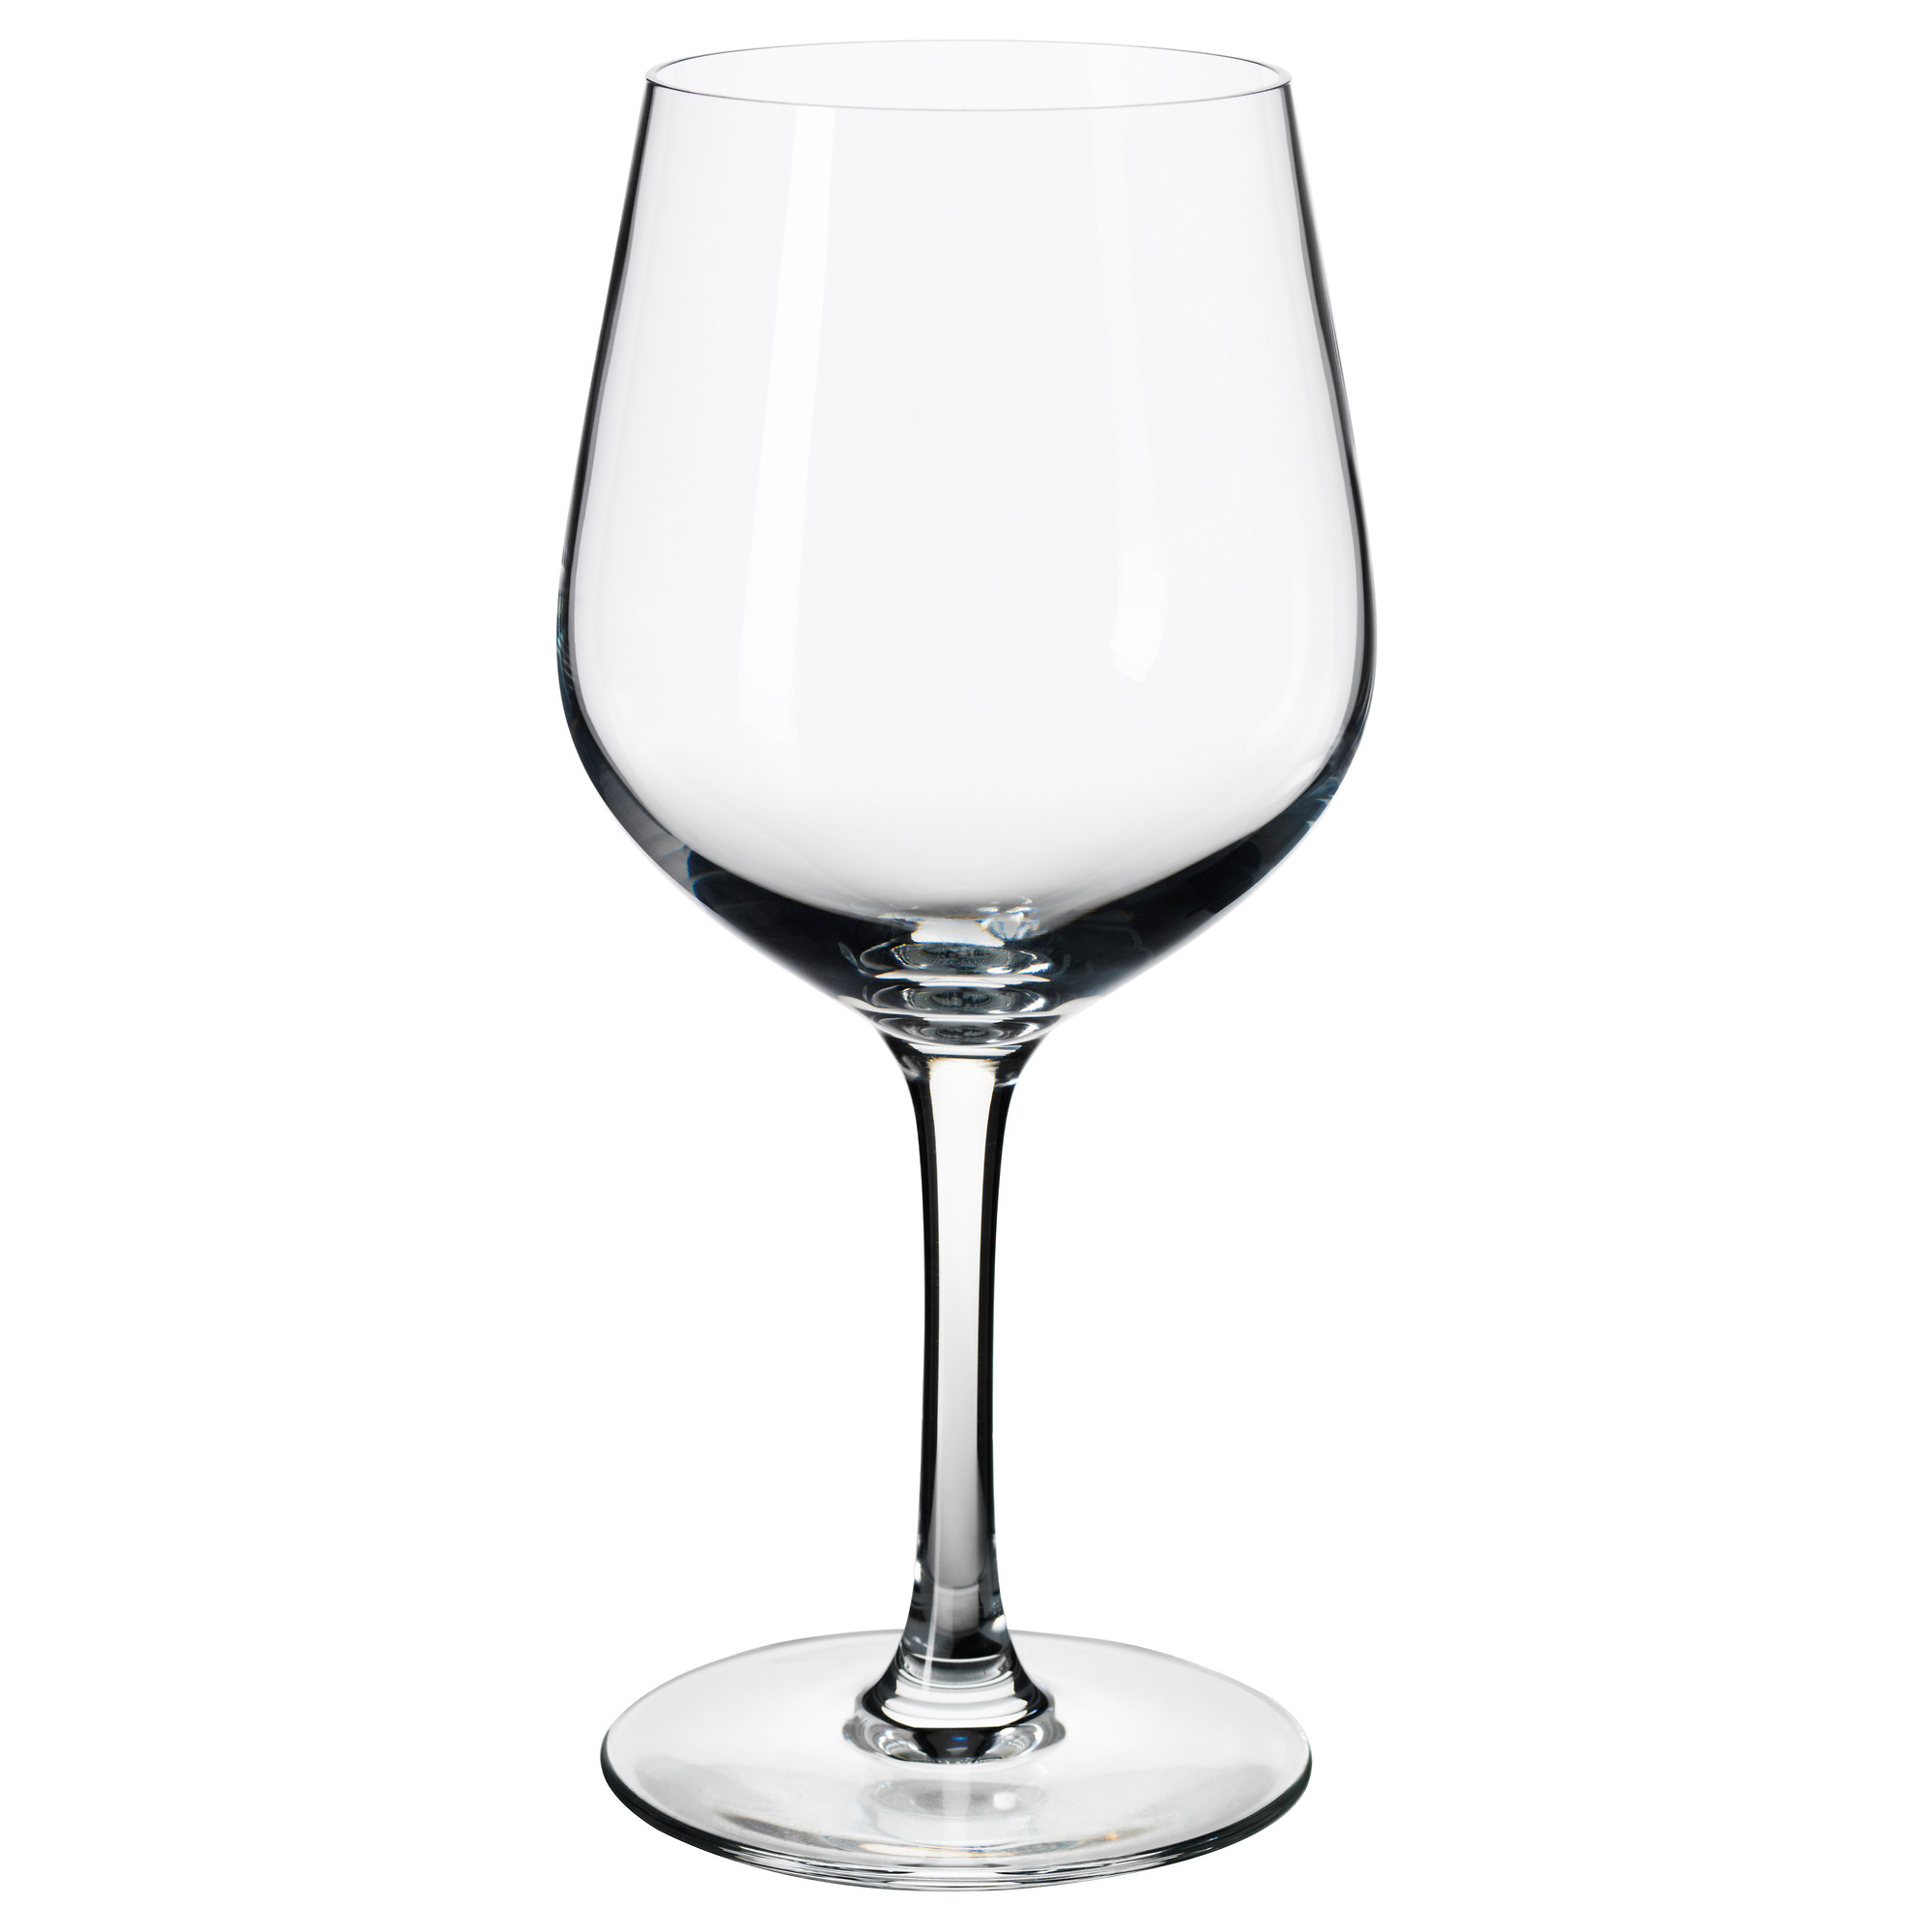
\includegraphics[width=0.382\textwidth]{pictures/glass}
  \end{center}
%\caption{Weinfass Halberstadt}
\end{wrapfigure}
Betrachtet man das Integral
$$\int_0^bx^2\;\mathrm{d}x,$$
und dazu Abbildung \ref{pyramide}, so kann der Wert des Integrals unmittelbar als Masszahl für einen Flächeninhalt interpretiert werden. Schraffiere ihn.

\begin{figure}
\scalebox{1}{
\begin{tikzpicture}[line cap=round,line join=round,>=triangle 45,x=0.8cm,y=0.5cm]
\draw[->,color=black] (-2.2,0) -- (5.86,0);
\foreach \x in {-2,-1,1,2,4,5}
\draw[shift={(\x,0)},color=black] (0pt,2pt) -- (0pt,-2pt) node[below] {\footnotesize $\x$};
\draw[color=black] (5.52,0.08) node [anchor=south west] {$x$};
\draw[->,color=black] (0,-1.02) -- (0,11.06);
\foreach \y in {-1,1,2,3,4,5,6,7,8,9,10}
\draw[shift={(0,\y)},color=black] (2pt,0pt) -- (-2pt,0pt) node[left] {\footnotesize $\y$};
\draw[color=black] (0.1,10.66) node [anchor=west] {$y$};
\draw[color=black] (0pt,-10pt) node[right] {\footnotesize $0$};
\clip(-2.2,-1.02) rectangle (5.86,11.06);
\draw[smooth,samples=100,domain=-2.2:5.86] plot(\x,{\x^2});
\draw (3,9)-- (3,0);
\draw (2.8,-0.1) node[anchor=north west] {$b$};
\end{tikzpicture}
\begin{tikzpicture}[line cap=round,line join=round,>=triangle 45,x=0.8cm,y=0.8cm]
\draw[->,color=black] (-3.6,0) -- (5.6,0);
\foreach \x in {1.17,2.33,3.5,4.67}
\draw[shift={(\x,0)},color=black] (0pt,2pt) -- (0pt,-2pt);
\draw[->,color=black] (0,-2.96) -- (0,3.9);
\foreach \y in {-2,-1,1,2,3}
\draw[shift={(0,\y)},color=black] (2pt,0pt) -- (-2pt,0pt);
\clip(-3.6,-2.96) rectangle (5.6,3.9);
\draw [->] (3,2) -- (-3,-2);
\draw (0,0)-- (4,2);
\draw (4,2)-- (4,-1);
\draw (0,0)-- (3,1.2);
\draw (4,2)-- (3,1.2);
\draw (3,1.2)-- (3,-1.72);
\draw (4,-1)-- (3,-1.72);
\draw (0,0)-- (3,-1.72);
\draw [dotted] (0,0)-- (4,-1);
\draw (3.2,0) node[anchor=north west] {$b$};
\draw (5,-0.28) node[anchor=north west] {$x$};
\draw (-2.78,-2.02) node[anchor=north west] {$y$};
\draw (-0.5,3.6) node[anchor=north west] {$z$};
\end{tikzpicture}
}
\caption{Fläche $x^2$ und Grundfläche Pyramide}\label{pyramide}
\end{figure}

Betrachtet man aber dasselbe Integral zusammen mit der zweiten Figur, so identifiziert man den Integranden $x^2$ mit dem Flächeninhalt eines Quadrates der Seitenlänge $\abs{x}$, also als vertikalen Querschnitt einer quadratischen Pyramide an der Stelle $x$. Der Wert des Integrals erscheint jetzt als Volumen einer quadratischen Pyramide mit der Grundseite $b$ und der Höhe $b$.

Diese anschauliche Idee kann verallgemeinert werden, um das Volumen eines Körpers zu berechnen, der im xyz-Koordinatensystem zwischen den parallelen Ebenen $x = a$ und $x = b$ liegt.
Für jedes $x\in [a,b]$ sei die zugehörige Querschnittsfläche $Q(x)$ bekannt und die damit gebildete Funktion
$Q:x\mapsto Q(x)$ im Intervall $[a,b]$ stetig. Mit dieser Funktion $Q$ als Integrand lässt sich das Volumen $V$ des Körpers berechnen:
$$V=\int_a^bQ(x)\;\mathrm{d}x.$$

\begin{proof}[Beweis]
Offensichtlich ist $V(a) = 0$ und $V(b)$ der gesuchte Wert für das Volumen des Körpers.
Analog zu der Berechnung eines Flächeninhaltes werden wir im folgenden zeigen, dass auch zwischen den Funktionen $V$ und $Q$ ein wichtiger Zusammenhang besteht:
$$V'(x) = Q(x).$$
Das Volumen einer Scheibe lässt sich durch
$$V(x+h) - V(x)$$
angeben.

Im Intervall $[x,x+h]$ wird die Querschnittsfunktion $Q$ wegen ihrer Stetigkeit ein Minimum $Q_{min}$ und ein Maximum $Q_{max}$ annehmen. Auf diesen beiden Querschnittsflächen denkt man sich zwei Zylinder mit der Länge (Höhe) $h$, so dass sicher gilt:
$$Q_{min}\cdot h \leq V(x+h) - V(x) \leq Q_{max}\cdot h$$
und nach Division durch $h$
$$Q_{min} \leq \frac{V(x+h) - V(x)}{h} \leq Q_{max}$$
Wegen der vorausgesetzten Stetigkeit von $Q$ ist
$$\lim_{h\to0} Q_{min} = \lim_{h\to0} Q_{max} = Q(x).$$
Demnach existiert der Grenzwert
$$\lim_{h\to0}\frac{V(x+h) - V(x)}{h}$$
und sein Wert stimmt mit $Q(x)$ überein.
Mit anderen Worten: $V'(x) = Q(x)$, die Funktion $V$ ist eine Stammfunktion von $Q$. Schliesslich gilt wegen $V(a) = 0$ für das gesuchte Volumen
$$V = V(b) = V(b) - V(a) = V(x)|_a^b= \int_a^bQ(x)\;\mathrm{d}x.$$
\end{proof}

\begin{ueb}[Zylinder]
Ein Zylinder (Grundkreisradius $r$, Höhe $h$) liegt so im Koordinatensystem, dass die $x$-Achse zu seiner Mittelachse wird. Ermittle die Querschnittsfunktion $Q(x)$ und bestätige dann die Zylinderformel aus der Stereometrie.
\end{ueb}

\begin{ueb}[Kugel]
Der Ursprung des Koordinatensystems sei der Mittelpunkt einer Kugel mit dem Radius $r$. Zeige, dass $Q(x) = \pi(r^2 - x^2)$ und bestätige dann die Formel aus der Stereometrie.
\end{ueb}

\begin{ueb}[Kavalier der alten Schule]
 Begründe das Prinzip von \textsc{Cavalieri}: 
\begin{quote}
Stehen zwei Körper auf derselben Ebene und werden sie von jeder zu ihr parallelen Ebene in inhaltsgleichen Flächen geschnitten, so haben sie das gleiche Volumen.
\end{quote}
 \end{ueb}
 
 \subsection{Rotationsvolumen}
 Der Graph einer im Intervall $[a,b]$ stetigen Funktion $f$ mit $f(x)\geq0$ für alle $x\in [a,b]$ rotiere um die x-Achse.
Die Querschnittsfläche an der Stelle $x$ des so entstehenden Rotationskörpers ist inhaltsgleich der Fläche eines Kreises mit dem Radius $f(x)$:
$$Q(x)=\pi\left[f(x)\right]^2.$$
\begin{figure}
\begin{center}
 \scalebox{1.1}{
\definecolor{ffzzqq}{rgb}{1,0.6,0}
\begin{tikzpicture}[line cap=round,line join=round,>=triangle 45,x=0.6cm,y=0.6cm]
\draw[->,color=black] (-1.7,0) -- (10,0);
\foreach \x in {-1,1,2,3,4,5,6,7,8,9}
\draw[shift={(\x,0)},color=black] (0pt,-2pt);
\draw[color=black] (9.66,0.08) node [anchor=south west] {$x$};
\draw[->,color=black] (0,-3.72) -- (0,3.98);
\foreach \y in {-3,-2,-1,1,2,3}
\draw[shift={(0,\y)},color=black] (-2pt,0pt);
\draw[color=black] (0.1,3.58) node [anchor=west] {$y$};
\clip(-1.7,-3.72) rectangle (10,3.98);
\draw[line width=2pt, smooth,samples=100,domain=1.0:8.0] plot(\x,{0-(0.05)*(\x-4.5)^2+3});
\draw [dash pattern=on 3pt off 3pt] (1,2.39)-- (1,0);
\draw [dash pattern=on 3pt off 3pt] (3,2.89)-- (3,0);
\draw [dash pattern=on 3pt off 3pt] (8,2.39)-- (8,0);
\draw[line width=2pt, smooth,samples=100,domain=1.0:8.0] plot(\x,{0.05*(\x-4.5)^2-3});
\draw [rotate around={90:(1,0)},line width=2pt] (1,0) ellipse (1.442cm and 0.396cm);
\draw [rotate around={90:(3,0)},line width=2pt,color=ffzzqq,fill=ffzzqq,fill opacity=0.2] (3,0) ellipse (1.722cm and 0.432cm);
\draw [rotate around={90:(8,0)},line width=2pt] (8,0) ellipse (1.442cm and 0.432cm);
\draw[color=black] (1.22,2.94) node {$f$};
\draw[color=black] (0.96,-0.24) node {$a$};
\draw[color=black] (3,-0.24) node {$x$};
\draw[color=black] (3.7,1.3) node {$f(x)$};
\draw[color=black] (7.96,-0.24) node {$b$};
\end{tikzpicture}
}
\end{center}
\caption{Rotationsvolumen}
\end{figure}

Für das Volumen des Rotationskörpers gilt demnach:
$$V(x)=\pi\int_a^b\left[f(x)\right]^2\;\mathrm{d}x.$$

\begin{ueb}[checkmate!]
Berechne das Volumen
\begin{enumeratea}
\item eines senkrechten Kreiskegels mit dem Grundkreisradius $r$ und der Höhe $h$,
\item eines Kegelstumpfes mit den Radien $R$ und $r$ und der Höhe $h$,
\item einer Kugel mit dem Radius $r$,
\item eines Kugelsegmentes mit dem Kugelradius $R$ und der Höhe $h$.
\end{enumeratea}
\end{ueb}

\begin{ueb}[hyperbolisch]
Zeichne in einem Koordinatensystem die Hyperbel mit der Gleichung $y=\frac{1}{x}$. Die durch die $x$-Achse, die Geraden mit den Gleichungen $x = 1$ und $x = b$, $b>1$ und die Hyperbel begrenzte Fläche rotiere um die x-Achse. Berechne das Volumen $V(b)$ des Rotationskörpers. Gegen welchen Wert strebt $V(b)$ für $b\to\infty$? Beachte, dass dieser \glqq Grenzkörper\grqq\ eine unendlich grosse Oberfläche hat.
\end{ueb}

\begin{ueb}[in vinos veritas]
Ein Fass wird sehr gut durch ein zwischen zwei Grenzen um die $x$-Achse rotierendes Parabelstück beschrieben. Dabei hat die Parabel die Gleichung $y = - ax^2+b$. Ein Fass hat die Länge (Höhe) $\unit[1]{m}$; der Durchmesser der Boden- bzw. Deckfläche beträgt $\unit[60]{cm}$ und sein grösster Durchmesser $\unit[80]{cm}$. Berechne den Rauminhalt des Fasses.
\end{ueb}

\begin{ueb}[Tropf]
Der
\marginnote{
\qrcode{
https://www.youtube.com/watch?v=Q7dnCyl_zUY}
}
Die Randfunktion eines Stromlinienkörpers wird durch die Gleichung
$$f(x)=\frac{1}{4}(4-x)\sqrt{x}.$$
zwischen $x = 0$ und $x = 4$ erfasst. Skizziere den Körper, berechne seinen grössten Durchmesser und sein Volumen.
\end{ueb}

\begin{ueb}[Träne]
\ \\[-4ex]
\begin{enumeratea}
\item Durch Drehung der Sinuskurve $y = \sin x$ zwischen $x = 0$ und $x = \pi$ um die $x$-Achse entsteht ein spindeIförmiger Körper, dessen Volumen zu berechnen ist.
\item Der Graph der Funktion
$$f(x)=1+\sin(x)\q(0<x<\frac{3\pi}{2})$$
schliesst mit den Koordinatenachsen ein Flächenstück ein, das um die $x$-Achse rotiert. Berechne das Volumen dieser \glqq Zwiebelhaube\grqq.
\end{enumeratea}
\end{ueb}

\newpage

\appendix

\section{Partielle Integration}

\begin{wrapfigure}{r}{0.382\textwidth}
\vspace{-12pt}
  \begin{center}
    \includegraphics[width=0.38\textwidth]{pictures/integrieren}
  \end{center}
%\caption{You Know my Name}
\vspace{-18pt}
\end{wrapfigure}
Wenn man sich mit komplexeren Funktionen konfrontiert sieht, insbesondere mit Produkten, dann kann folgendes Hilfsmittel zur Bestimmung des Integrals nützlich sein.

\begin{csatz}[Partielle Integration]{satz:partint}
Sind $f$ und $g$ \glqq an der Stelle $x$ differenzierbare Funktionen, so gilt
$$\int f'(x)g(x) = f(x)g(x) - \int f(x)g'(x)$$
\end{csatz}

\begin{proof}[Beweis]
Für einen Beweis beachte man die Ähnlichkeit zur bereits bewiesenen Produktregel für Ableitungen und argumentiere.
\end{proof}

\begin{bsp}
Wir bestimmen via partielle Integration eine Stammfunktion von $h(x)=x\cos(x)$. Setzen wir beispielsweise $\cos(x)=f'(x)$ und $x=g(x)$, dann gilt $f(x)=\sin(x)$ und $g'(x)=1$. Daraus folgt

\begin{align*}
 \int x\cos(x)\;\mathrm{d}x &= x\sin(x)-\int\sin(x)\;\mathrm{d}x\\
 &=x\sin(x)-(-\cos(x))+c\\
 &=x\sin(x)+\cos(x)+c.
 \end{align*}
 
Man kontrolliert durch Ableiten der eben gewonnen Stammfunktion die Korrektheit.
\end{bsp}

\begin{ueb}[partiell, and again]
Finde eine Stammfunktion von $f(x)=x\sin(x)$, $g(x)=\sin^2(x)$ und $h(x)=\sin^3(x)$. Bei $h$ \glqq spüren\grqq\ Sie erstmals, wie viel Aufwand das Finden von Stammfunktionen bescheren kann!
\end{ueb}

\pagebreak

\section{Kepler'sche Fassregel}

\begin{wrapfigure}{r}{0.382\textwidth}
\vspace{-5pt}
  \begin{center}
    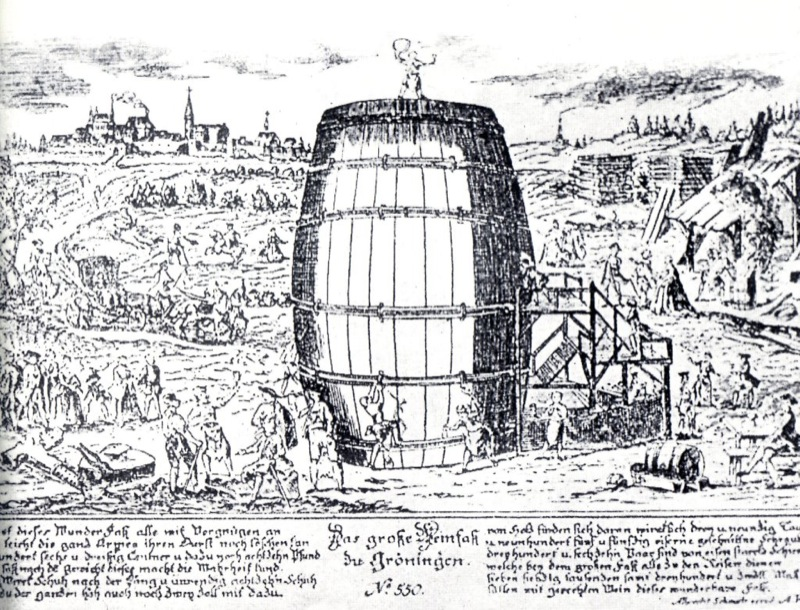
\includegraphics[width=0.38\textwidth]{pictures/weinfass}
  \end{center}
\caption{Weinfass Halberstadt}
\vspace{-10pt}
\end{wrapfigure}
Die Keplersche Fassregel ist die einfachste, aber dennoch brauchbare Resultate liefernde Regel für die näherungsweise Berechnung eines bestimmten Integrals.
\textsc{Johannes Kepler} erzählt in seinem Buch \glqq Neue Stereometrie der Weinfässer\grqq:
\begin{quote}
Als ich im November des letzten Jahres (1613) meine Wiedervermählung feierte, zu einer Zeit, da an den Donauufern bei Linz die aus Niederösterreich herbeigeführten Weinfässer nach einer reichlichen Weinlese aufgestapelt und zu einem annehmbaren Preis zu kaufen waren, da war es die Pflicht des neuen Gatten und sorglichen Familienvaters, für sein Haus den nötigen Trunk zu besorgen. Als einige Fässer eingekellert waren, kam am 4. Tag der Verkäufer mit der Messrute, mit der er alle Fässer, ohne Rücksicht auf ihre Form, ohne jede weitere Überlegung oder Rechnung ihrem Inhalt nach bestimmte\dots. Ich bezweifelte die Richtigkeit der Methode, denn ein sehr niedriges Fass mit etwas breitem Boden und daher sehr viel kleinerem Inhalt könnte dieselbe Visierlänge besitzen. Es schien mir als Neuvermählter nicht unzweckmässig, ein neues Prinzip mathematischer Arbeiten, nämlich die Genauigkeit dieser bequemen und allgemein wichtigen Bestimmung nach geometrischen Grundsätzen zu erforschen und die etwa vorhandenen Gesetze ans Licht zu bringen.\grqq
\end{quote}

Die Keplersche Fassregel erwies sich später als ein Spezialfall der Simpsonregel für n = 2. Man erhält so mit Hilfe geometrischer Überlegungen (vgl. auch Abbildung \ref{abb:fass} auf Seite \pageref{abb:fass}).
$$
\int_a^bf(x)\;\mathrm{d}x\approx K =\frac{b-a}{6}\left[f(a)+4f\left(\frac{a+b}{2}\right)+f(b)\right].
$$

\begin{bem}
Für ganzrationale Funktionen von höchstens 3. Grad gibt $K$ sogar den exakten Wert an.
\end{bem}

\begin{ueb}[Rollt das Fass rein!]
Wende die Keplersche Fassregel an auf das Integral

\begin{minipage}{3.8cm}
\begin{enumeratea}
\item $\int_1^3x^2\;\mathrm{d}x$
\item $\int_0^\pi\sin x\;\mathrm{d}x$
\end{enumeratea}
\end{minipage}
\begin{minipage}{3.9cm}
\begin{enumeratea}
\addtocounter{enumi}{2}
\item $\int_1^2\frac{1}{x}\;\mathrm{d}x$
\item $\int_0^1\frac{1}{1+x^2}\;\mathrm{d}x\q$
\end{enumeratea}
\end{minipage}

\vspace*{2ex}
Vergleiche die Resultate mit dem exakten Wert.
\end{ueb}

\begin{figure}
\begin{center}
\scalebox{1.3}{
\begin{tikzpicture}[line cap=round,line join=round,>=triangle 45,x=0.6cm,y=0.5cm]
\draw[->,color=black] (-0.72,0) -- (10.3,0);
\foreach \x in {,1,2,3,4,5,6,7,8,9,10}
\draw[shift={(\x,0)},color=black] (0pt,-2pt);
\draw[color=black] (9.96,0.08) node [anchor=south west] {$x$};
\draw[->,color=black] (0,-1.22) -- (0,5.24);
\foreach \y in {-1,1,2,3,4,5}
\draw[shift={(0,\y)},color=black] (-2pt,0pt);
\draw[color=black] (0.1,4.84) node [anchor=west] {$y$};
\clip(-0.72,-1.22) rectangle (10.3,5.24);
\draw[line width=1.6pt, smooth,samples=100,domain=1.0:9.0] plot(\x,{0-(0.05)*(\x-6)^2+4});
\draw (1.5,2.99)-- (1.5,0);
\draw [dash pattern=on 4pt off 4pt] (4.5,3.89)-- (4.5,0);
\draw (7.5,3.89)-- (7.5,0);
\draw (1.68,1.86) node[anchor=north west] {$f(a)$};
\draw (1.08,-0.1) node[anchor=north west] {$x_0=a$};
\draw (3.86,0.12) node[anchor=north west] {$x_1=\frac{a+b}{2}$};
\draw (7.12,0) node[anchor=north west] {$x_2=b$};
\draw (4.7,2.6) node[anchor=north west] {$f\left(\frac{a+b}{2}\right)$};
\draw (7.68,2.24) node[anchor=north west] {$f(b)$};
\draw[color=black] (1.14,3.34) node {$f$};
\end{tikzpicture}
}
\end{center}
\caption{Keplersche Fassregel}\label{abb:fass}
\end{figure}

\cleardoublepage
\listoffigures
%\listoftables
%\newpage
%\nocite{*}
%\bibliographystyle{plain}
%\bibliography{preamble/literaturgoogle}
\end{document}